\documentclass[12pt]{article}
\usepackage[T1]{fontenc}
\usepackage{geometry}
\geometry{verbose,tmargin=0.5in,bmargin=0.75in,lmargin=0.75in,rmargin=0.5in}
\pagestyle{headings}
\usepackage{color}
\usepackage{ragged2e}
\usepackage{graphics}
\usepackage{graphicx}
\newcommand{\versionnumber}{3.2}
\makeatletter


\begin{document}

\title{Beamline Manual\\\normalsize Version \versionnumber}
\author{S. Stepanyan, E. Pasyuk}
\maketitle



\section{Contacts\label{beamline_contacts}}

\begin{description}
\item [Beamline~cell phone] (757) 303-3996
\end{description}

Personnel listed in Table \ref{tab:calllist} should be called whenever there
is a problem beyond the on-hand expertise. The beam line expert is the main source for help.  
\begin{table}[tbhp]
\vspace{0.3cm}
{\centering \begin{tabular}{|c|c|c|c|}
\hline 
Who&Expertise&Cell Phone&Office\\
\hline 
\hline 
MCC&Beam tune, vacuum&&x7048 \& x7043\\
\hline 
Expert on call&Beamline devices and applications&(757) 303-3996&\\
\hline 
Eugene Pasyuk&Beamline devices and applications&(757) 515-9811&x6020\\
\hline 
Engineering on call&General beamline&(757) 748-5048&\\
\hline 
\end{tabular}\par}
\vspace{0.3cm}


\caption{The beamline call list.\label{tab:calllist}}
\end{table} 



\section{What to Monitor along the Beamline}


\subsection{Beam conditions}
\indent

During data taking it is important to monitor electron beam
to insure that there are no changes in the beam parameters which can effect quality of data. For
example, changes in the beam halo can dramatically increase background rates
making the data worthless, or a change in the electron beam direction can cause
unwanted beam losses leading detector damage or beam trip. There are
automatic controls and alarms for the beam conditions that will prevent beam damage to equipment 
and will terminate beam delivery in an event of beam excursions. Nevertheless,  the shift taker must
continuously monitor the beam parameters and act accordingly.

After the initial beam tune, reference numbers for the beam parameters (position of the beam on position monitors, i.e. BPMs) and the rates of halo counters will be posted in the log book and on the run wiki page, and must be used as reference. 

\subsubsection{Beam Current}
\indent

A consistency in the beam current readings between the Faraday Cup (see Section \ref{sec:fcup}) and the "nA" BPMs is one way
to check that the electron beam is cleanly transported to the beam dump (Faraday Cup). {\bf Note:} for most of CLAS12 experiments, requested beam current (at nominal luminosity) exceeds allowed power limit for the Faraday cup, $\sim 175$ W (Power in W = Current in nA x Energy in GeV). A beam blocker, see Section \ref{subsec:blocker}, will be inserted in front of the Faraday cup. Even with blocker in-beam, Faraday cup reading is meaningful, it will be a scaled value of the beam current. The coefficient of the proportionality is beam energy dependent \cite{blocker} and will be calibrated at each given energy setting \cite{2018-003}. With blocker in-beam, the ratio of the currents read by Faraday cup and other current monitors (e.g. BPMs, Section \ref{sec:bpm}, and SLM, Section \ref{sec:slm}) must be constant. In all cases one should observe the same current on all three nA BPMs (2C21, 2C24, and 2H01). In addition to the inconsistencies in the beam current readings, the halo counters (see Section \ref{sec:scaler_a}) should
show an increased activity if beam scraps beam pipes. Also higher then normal rates in the detectors would be indicative
of scraping immediately downstream of the target.

In the event that there appears to be unacceptable beam losses the following course of action is recommended:

\begin{enumerate}
\item Stop beam delivery and data taking, make a log entry flagging any data runs that may have been
affected.
\item Call MCC and explain to the operator what has been observed and explain why
the tune is unacceptable.
\item Work with the MCC operator to come up with a game plan to fix the problem.
\item Document the solution and start taking data again.
\end{enumerate}


\subsubsection{Beam Halo}
\indent

The presence of a beam halo is usually observed by an increase count rate in
the beam halo counters (see Section \ref{sec:scaler_a}). Typically
the upstream and midstream counters are very quiet. Any count rate above $\sim$tens of Hz (after initial gain adjustments for a well tuned beam) is indicative
of a problem. Note that an increase count rate in the upstream beam halo counters
can also indicate an obstacle on the beam path or just a bad beam tune. To 
further investigate the source of a large count rate in the upstream beam halo
counters a harp scan (see the "electron beam profile scan" procedure in Section \ref{sec:harp}) should be performed. 

If the beam halo is unacceptable, take the following steps:

\begin{enumerate}
\item Stop beam delivery and data taking, make a log entry.
\item Call MCC and explain to the operator what has been observed and why this tune
is unacceptable.
\item Work with MCC to solve the problem.
\item Document the solution and start taking data again.
\end{enumerate}

\subsubsection{Beam Position}
\indent

The beam position before CLAS12 is available from three "nA" cavities, 2C21, 2C24, and 2H01, and one stripline BPM, 2H00 (when beam current is above $25$ nA). The position monitors close to the target, 2H00 and 2H01, are the most important ones to keep the beam position steady on the target. A feedback system (the orbit locks) uses (x,y) positions on these BPMs, and the Horizontal and Vertical correctors on 2C22/2C23/2H00 girders to keep the beam position stable. Drifts more the \( \pm 0.2 \)mm
should be brought to the attention of MCC. The nA BPMs measure beam position as well as the current. Before data taking, shift worker must confirm that the feedback system is active (verify with MCC). Note, that at beam currents below $25$ nA only "nA" cavities are reliable. 

\subsection{Beamline Vacuum}
\indent

The beamline vacuum on Hall-B line (from upstream tunnel to the Faraday cup) can be monitored from the vacuum gauge readings available on the Main scaler GUI (see below). The vacuum upstream of the tagger magnet (upstream tunnel) usually is better than \( 10^{-6} \) torr , vacuum  downstream of the tagger magnet and in the downstream beam line it is usually better than \( 10^{-5} \) torr. Vacuum is tightly monitored and interlocked to the beam delivery. 


\subsubsection{Catastrophic Loss of Vacuum}
\indent

There are two thin windows that are components of the CLAS beamline, the target scattering chamber exit window
and the entrance window to the downstream beamline (after the target). If the window on the scattering chamber fails, fast valves interlocked to the pressure gauges will close automatically. These valves will limit the loss of the vacuum to a small region of the Hall B beamline. Valves are interlocked to the beam Fast Shutdown System (FSD) and beam will be terminated in an event of a vacuum loss.

If any of the valves close due to poor vacuum: 

\begin{enumerate}
\item notify MCC immediately, turn off the beam (if it is not already OFF)
\item call the engineering on call 
\end{enumerate}

If the window on the downstream beamline will fail, rates on the downstream halo counters will increase and will initiate FSD. 

\subsection{Magnet Power Supplies}
\indent

The Hall-B beamline and CLAS12 have magnets for beam transport, and momentum analysis. In Table \ref{magnets} the list of the magnets, their power supplies and point of control (POC) are shown. The items listed with B
as the point of control will be controlled by staff in the counting
house. The vertical and horizontal correctors, and the tagger magnet are controlled
by MCC, but the shift taker should monitor their settings. The tagger
magnet power supply is interlocked to the machine Fast Shutdown System (FSD). Interlocks are activated if run requires dumping the beam in the tagger beam dump, e,g during the initial beam tune or during the beam polarization measurements using the M{\"o}ller polarimeter. If the tagger
dipole power supply will trip, the beam will be automatically shut off. This interlock must 
be masked out when electron beam is delivered to the CLAS target. This is controlled in the BTA GUI by proper state of beam delivery, "photon" or "electron"). 

The CLAS12 solenoid is also interlocked to the machine Fast Shutdown System and must be activated (unmasked) when  electron beam is delivered to the CLAS12 target, to the electron dump (Faraday cup). 

\begin{table}[tbhp]
\vspace{0.3cm}
{\centering \begin{tabular}{|c|c|c|c|c|}
\hline 
magnet&
power supply&
POC&
Function&
Status\\
\hline 
\hline 
MB2C21V&
&
MCC&
vertical kick&
Active\\
\hline 
MB2C21H&
&
MCC&
horizontal kick&
Active\\
\hline 
m{\o}ller A&
Dyna-B&
B&
M{\o}ller polarimeter&
Not used\\
\hline 
m{\o}ller B&
Dyna-C&
B&
M{\o}ller polarimeter&
Not used\\
\hline 
MB2C22H&
&
MCC&
horizontal kick&
Active\\
\hline 
MB2C23V&
&
MCC&
vertical kick&
Active\\
\hline 
raster\_h1&
Danfysik&
B&
first horizontal target raster&
Not used\\
\hline 
raster\_v1&
Danfysik&
B&
first vertical target raster&
Not used\\
\hline 
tagger&
Danfysik&
MCC&
bend beam to tagger dump&
Active\\
\hline 
MBD2H00H&
&
MCC&
horizontal kick&
Active\\
\hline 
MBD2H00V&
&
MCC&
vertical kick&
Active\\
\hline 
Solenoid&
$-$&
B&
Moller shield and momentum analysis in CD&
Not used\\
\hline 
Torus&
Danfysik&
B&
CLAS12 FD spectrometer magnet&
Active\\
\hline 
\end{tabular}\par}
\vspace{0.3cm}


\caption{List of the magnets along the Hall B beamline and their functionality.\label{magnets}}
\end{table} 

If the tagger or any of CLAS12 superconducting magnets do trip off or is set incorrectly take the following action:

\begin{enumerate}
\item Call MCC immediately, tell them to shut off the beam (if it is not off already). Call Hall-B engineering on-call if torus or solenoid triped.
\item Make a log entry.
\item Restore magnets 
\begin{itemize}
\item have MCC restore the tagger dipole 

or 

\item call engineering on-call to restore CLAS12 superconducting magnets (torus or solenoid)
\end{itemize}
\item Restore beam, (if beam was going to Faraday cup, verify that the beam is incident on the downstream viewer on the same location as before the trip.)
\end{enumerate}

\subsection{Magnet and Power Supply Beacons}
\indent

Near every magnet in Hall B there is a \textcolor{red}{red flashing beacon} that indicates status of the magnets. If beacon is
flashing then the magnet \textbf{\textcolor{black}{is powered}} or \textbf{\textcolor{black}{can be powered}} at
any time. If you need to work near or on a magnet and the red light is flashing
you must turn off the supply. The dangers of working
near a magnet are limited to those associated with stray magnetic fields. All
the high current bus work is enclosed in protective shields so there is no shock
hazard. Of course the supply needs to be shut off, and locked and tagged before
any of the protective shield is removed.

After any work that required the power supply to be locked and tagged, a through
sweep of the magnet area for magnetic debris is required before the lock and
tag can be removed.


\section{Hall B Beamline devices and Epics Control Screens}

All the GUIs necessary to control and monitor beam line devices and the CLAS12 detector can be launched from CS Studio EPICS interface. 

\subsection{EPICS GUI Launcher}
\indent

The \emph{"clascss"} (see Fig.\ref{clascss}) is a \emph{css studio} screen that serves as an icon manager of
\emph{css} GUIs. From this screen, the bulk of the epics applications can
be started. It is recommended that when finished with a particular \emph{css}
screen, that application be terminated (\textbf{not iconized}). If the screen
is needed in the future, just launch it again from the \emph{"clascss"}. In this
manner, searching through all the degenerate icons is eliminated. 

To start the \emph{"clascss"}:

\begin{itemize}
\item log on one of  \textbf{clon} PCs or \textbf{clonsl(1,2,3)} computers as clasrun
\item type: \textbf{clascss}
\end{itemize}

\begin{figure}[htp]
{\centering 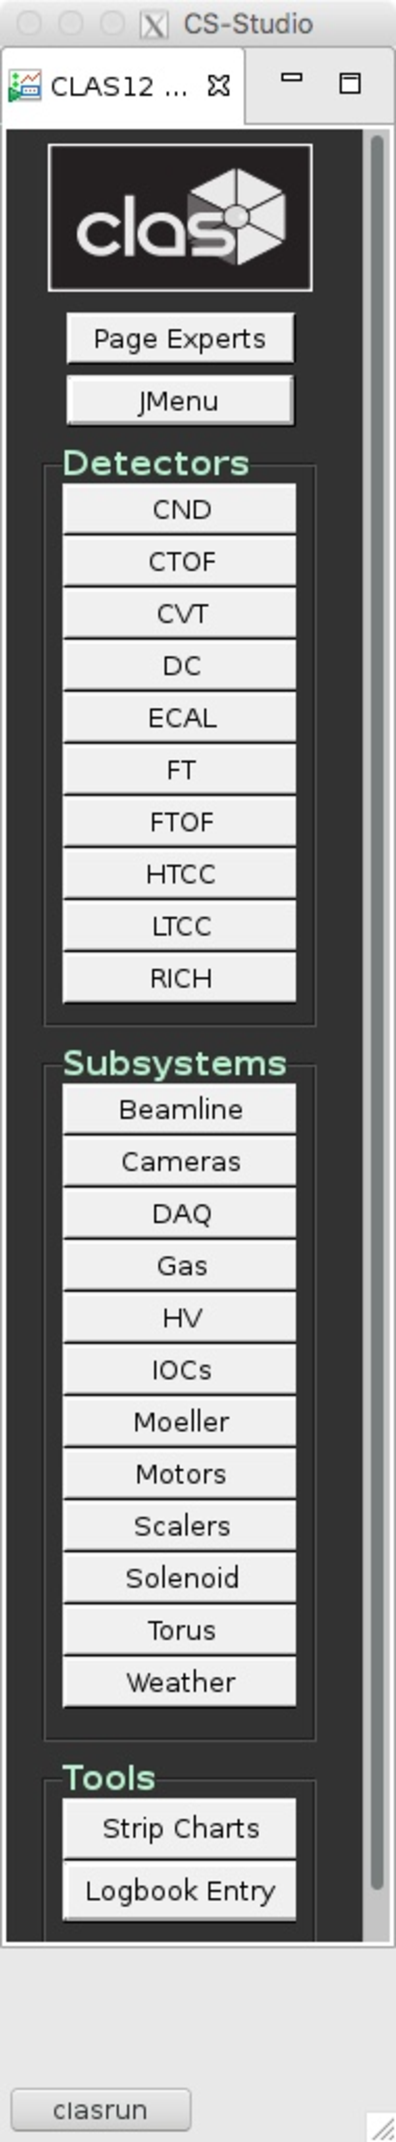
\includegraphics[scale=0.65]{CLAS_CSS.pdf}\par}
\caption{\small{CLAS12 EPICS GUI launcher.}}
\label{clascss}
\end{figure}

Most of the beamline applications are under the \emph{"Beamline"} pull down menu. The beamline devices that have motor controls can be found under \emph{"Motors"} pull down menu, scalers under \emph{"Scalers"}, the M{\o}ller polarimeter controls under \emph{Moeller}.  

\subsection{The Main Control and Monitoring Screen}
\indent

The most relevant information for running the beam in a safe and efficient manner is displayed and can be controlled from the Main Control and Monitoring GUI, see Figure \ref{fig:scaler}. This screen can be launch from CS-studio interface using \emph{"Beamline"} button from the menu. The main control screen should be up on a single display on one of PCs in the counting room and must be monitored by shift personnel at all times. 

The GUI consists of several rows of information. On the top row rates in the beam halo counters and in the CLAS12 detector elements are displayed. The second row displays information on the beam position (BPM, BOM) and current (BPM, SLM, Faraday cup) monitors, and on the CLAS12 target. The middle row has all moving devices, harps, the collimator, beam viewer, and beam blocker. In row four, vacuum gauges (cold cathode gauges) are displayed. The bottom row shows magnet settings, including correctors, quadrupoles, the tagger dipole and the CLAS12 solenoid and torus.  In addition, there are information about the beam, its destination, energy, on helicity related parameters, and the beam viewer in the downstream tunnel.


\begin{figure}[tbhp]
{\centering \resizebox*{0.75\textwidth}{!}{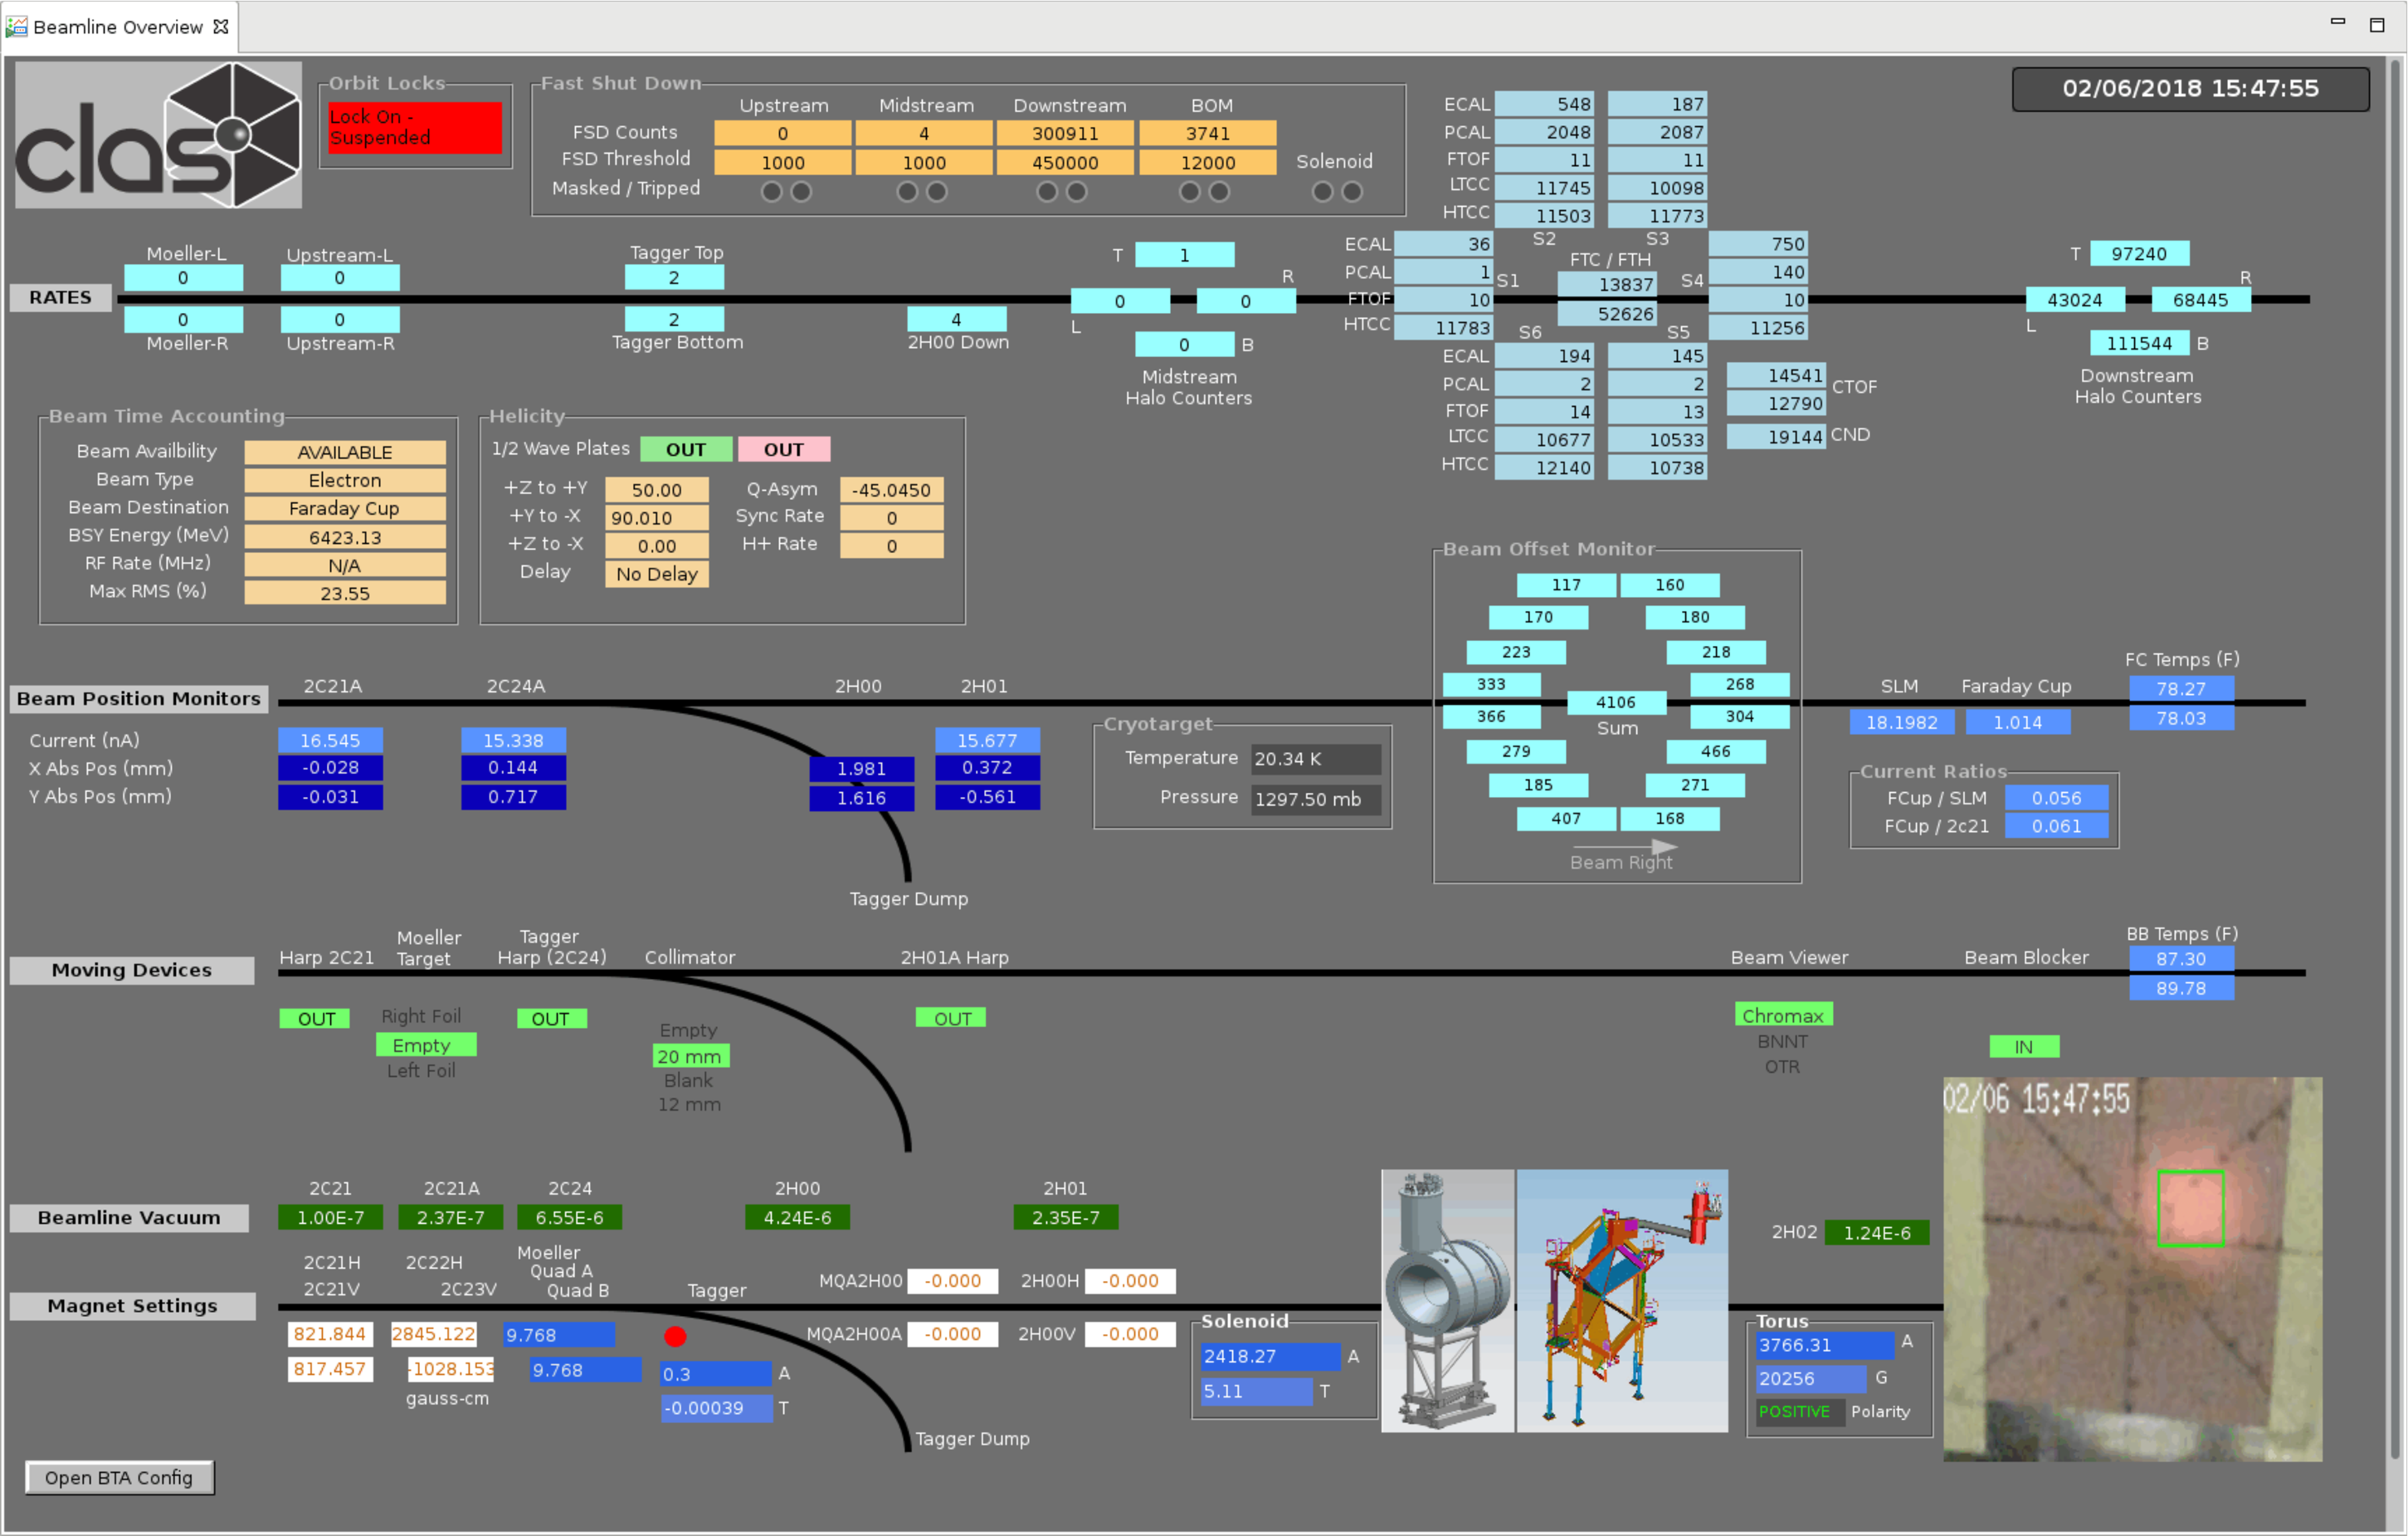
\includegraphics[angle=90]{main_scaler_gui.pdf}} \par}
\caption{The main scaler GUI.}
 \label{fig:scaler}
\end{figure}

\subsection{Beam Halo Counters (classc1/classc4) \label{sec:scaler_a}}
\indent

The beam halo counters consist of photomultiplier tubes with plastic attached to their photocathodes strapped to the beam pipes along the beamline. There are two halo counters upstream of the Hall-B tagger magnet, \emph{Upstream-L} and \emph{Upstream-R}, two on the top and bottom of the tagger magnet, \emph{Tagger Top} and \emph{Tagger Bottom}, one downstream of the collimator box, \emph{2H00 Down}, four counters upstream of the CLAS target, \emph{Midstream L/R/T/B}, and four counters located in the apex of the forward carriage, \emph{Downstream L/R/T/B}. The beam halo counter scalers are displayed on the Main GUI, top line. HV control of these PMTs can be opened from \emph{"Beamline"} menu.

The rates in halo counters are good indicators of the beam transport quality. After initial beam tune and calibration, rates for good beam conditions will be recorded in the logbook and on the run wiki, and should be closely monitored. 

\subsubsection{Beam Offset Monitor}
\indent

In addition to the halo counters, there is a beam offset monitor (BOM) mounted upstream of the target, centered on the entrance window of the target cell. The BOM consists of a glass-silica cylinder ($10$ mm ID) with $16$ plastic fibers attached to the upstream perimeter. A 2 meters long fibers are uniformly distributed along the perimeter of the cylinder, routed outside of the beam vacuum and read out with multi-anode (16) Hamamatsu PMT. 

The main function of the BOM is to alert on beam motion at the target. If beam moves from the target center it will generate high rates in BOM PMT due to interaction of the beam tails with quartz cylinder. 


\subsection{BPMs}
\label{sec:bpm}
\indent

There are 3 nA Beam Position Monitors (BPMs), 2C21, 2C24 and 2H01, and one stripline BPM 2H00 on the B-line. The nA BPMs measure beam transfer (x,y) position relative to their center as well as the beam current. The stripline BPM measures beam position and is reliable only for beam currents above $25$ nA. There is a BPM alarm GUI, Fig. 3,
that allows to set limits for beam position and current drifts from the requested values. The GUI can be open from the \emph{"Beamline"} pull down menu.
\begin{figure}[tbhp]
{\centering 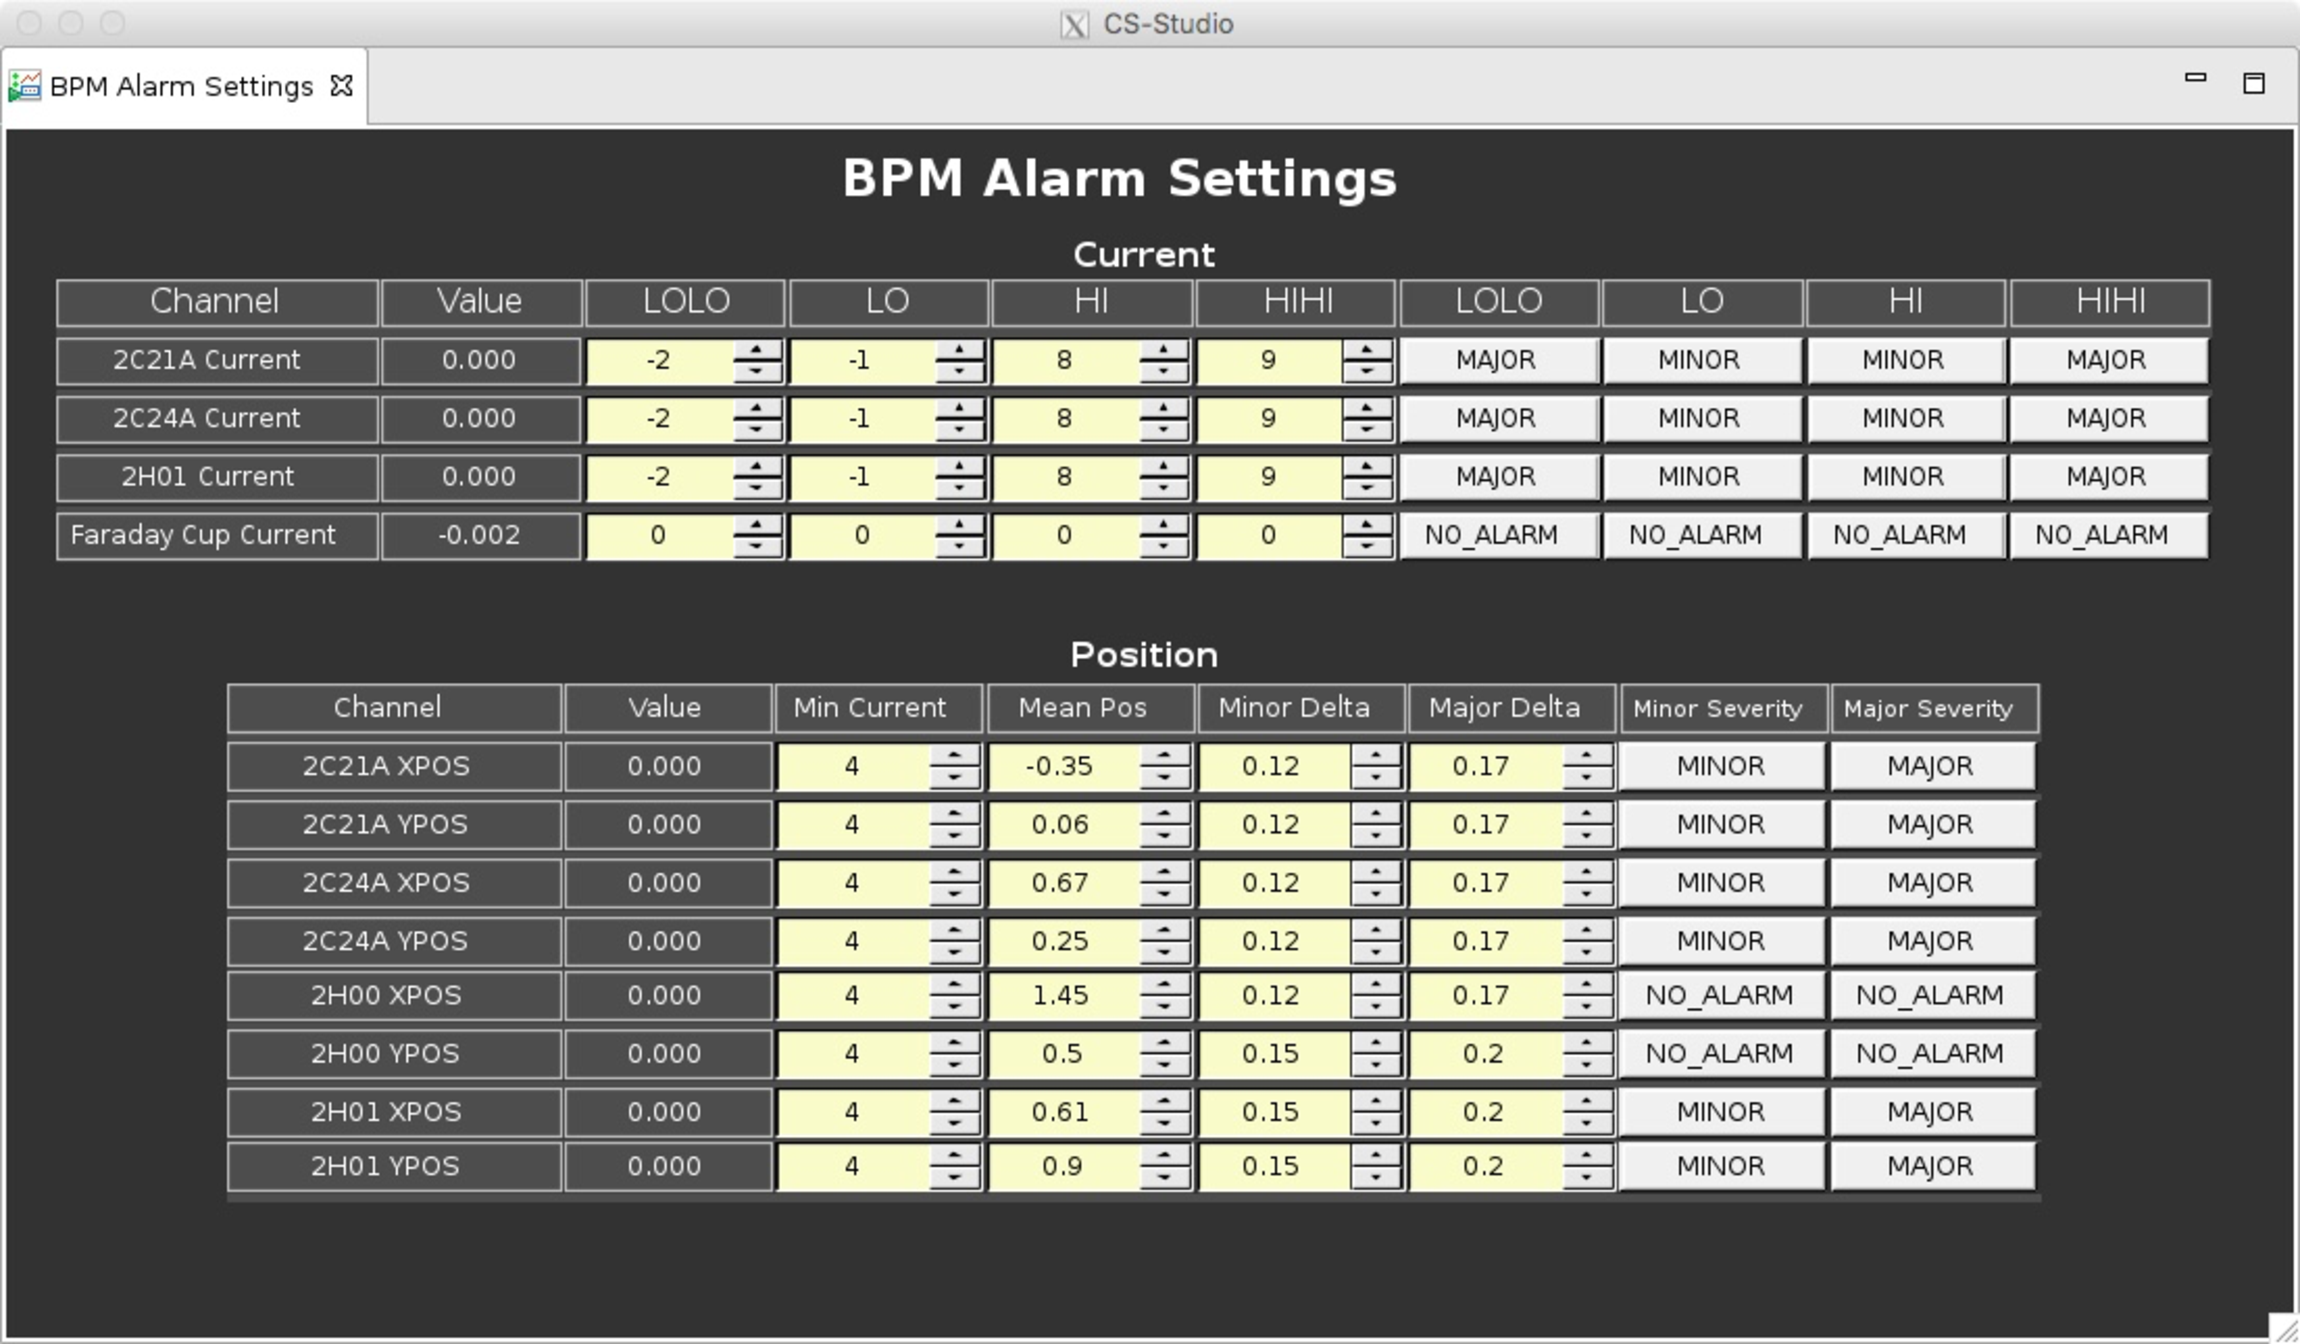
\includegraphics[scale=0.5, angle=90]{bpms.pdf} \par}
\caption{The Hall B BPM setup screen. The current reading, in nAmps. The Faraday Cup current
reading is updated at the same rate as the beam halo scalers. \label{fig:bpm}}
\end{figure}

\subsection{Hall-B Harps (classc3/classc4)\label{sec:harp}}
\indent

There are three wire harps on the Hall B beamline, 2C21, 2C24 ("tagger"), and 2H01A. The 2C21 harp has two $25~\mu$m tungsten wires that cross the beam in horizontal (X) and vertical (Y)directions. The "tagger" and 2H01A harps have two sets of wires, thin and thick. There are three thin $25~\mu$m tungsten wires, which cross the beam in X, Y, and $45^\circ$ axis. This are the main set of wires on these two harps that are used to perform beam profile measurements. Two thick wires ($1$ mm iron on 2C24 and 0.5 mm carbon on 2H01A) that are mounted farther from the beam, move into beam in X and Y directions and are used only for special measurements of the beam tails. The harp launch GUI, {\it Harp Scans} shown in Figure \ref{harpmain}, enables operator to open controls for the desired harp. Position of the stepper motor that moves the wires in conjunction
with the beam halo scalers is used to perform the beam profile measurements. The harp operation is controlled from the {\it Harp Scans} GUI (controls for 2C21 harp are shown on the figure). During the scan the scaler readout is controlled by the scan application,  (see Section \ref{sec:scaler_a}).

\begin{figure}[tbhp]
{\centering \resizebox*{0.75\textwidth}{!}{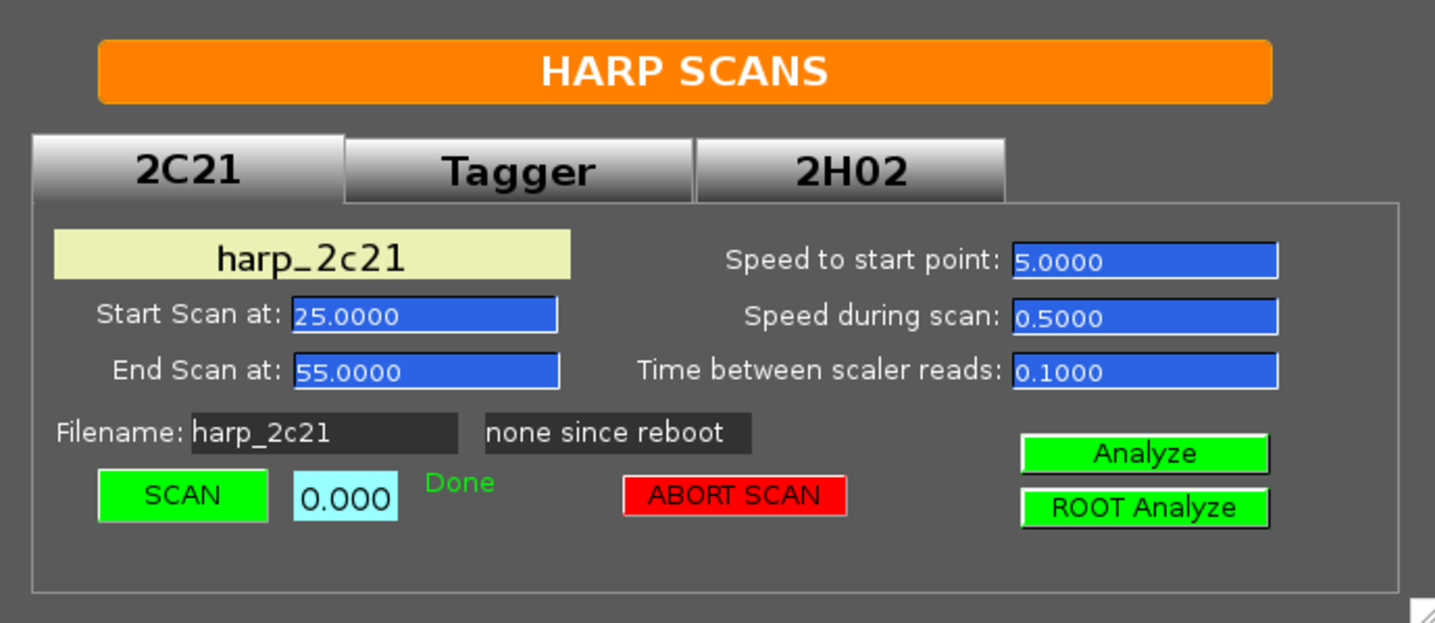
\includegraphics{harps.pdf}} \par}
\caption{The main Harp medm screen. The green buttons on the top are for opening individual harp control. Cyan buttons below for expert GUIs.}
\label{harpmain}
\end{figure}

In order to perform a harp scan one should push {\it SCAN} button. After the scan is finished (motor position has been restored at $0.0$) use {\it Analyze} button to see the beam profile and fit the halo counter rate as a function of the wire position. Make sure beam is stable during the scan. If beam has been lost during the scan (e.g. due to beam trips), information (halo counter rates) from wire crossing the beam will be lost. In this case beam scan must be repeated.  


\subsection{Collimator \label{sec:colim}}
\indent

In order to prevent direct beam exposure of the SVT or forward MM tracker in an event of beam excursions, a collimator is installed $\sim 15$ meters upstream of the detectors. This is the same collimator box and a $20$ cm long Nickel collimators that have been used in the past for the tagged photon beams in Hall B. One of collimators has been resized to have $20$ mm diameter hole. The collimator control GUI will have sizes and motor positions for each collimator in the box, see Figure \ref{fig:beamblocker}. In order to position required collimator open the {\it Motors} GUI, select {\it Hall-B Colli} tab and click on the collimator button you want to move.   

\subsection{Synchrotron Light Monitor \label{sec:slm}}
\indent

Synchrotron light monitor (SLM) is a PMT device that measures amount of synchrotron light generated by electron beam in the magnetic field of the last dipole right before the Hall-B upstream tunnel (when beam gets to the hall beamline elevation level). The synchrotron light device, nomenclature name 2C20, is composed of a mirror and a prism that splits the synchrotron light image in two. One is used by accelerator operations as beam viewer, another is directed to a 2" PMT and read out  on current integrator. The PMT signal is used by Hall-B as beam current monitor.   

The main use of this current monitor is to measure helicity related beam intensity (charge) asymmetry. While PMT signal strength depends on the beam position, for fast ($>$Hz) asymmetry measurements it works well without any corrections for position drifts, since position drifts are usually very slow process. Position dependence can be corrected using the 2C21 BPM position readout and in principal this device can be used for beam charge accounting if needed.    

\subsection{Beam Viewer \label{sec:view}}
\indent

There is a beam viewer installed in the downstream tunnel, right before the shielding wall that separates Faraday cup dump. The viewer is a wheel with a Chromox screen mounted on the axis. The motor that control the position of the screens can be controlled from the same {\it Motors} GUI as collimator, see Figure \ref{fig:beamblocker}. In order to position the screen just push the button carrying the name of the screen.  

\subsection{Faraday Cup (classc4) \label{sec:fcup}}
\indent

The instantaneous beam current reading from the Faraday cup is available on
the \textbf{Main Scaler} screen as shown in Figure \ref{fig:scaler}. The update rate is the same as for the beam halo scalers and
is controlled from the scaler GUI, see Section \ref{sec:scaler_a}. An important consideration
is that the Faraday Cup current integrater rate is $906.2$ counts/sec for 1 nA. This means that if the count time on the scaler is much less than 1 sec
you will observe large statistical fluctuations.


\subsubsection{Beam blocker}
\label{subsec:blocker}
\indent

The Hall-B Faraday cup is not cooled and cannot operate at high currents (deposited hit should not exceed $175$ W for more than 1/2 hour running). If run requires use of beam currents above the limit (for 11 GeV it is 15 nA), a $5$ kW beam blocker, cooled-copper absorber, must be position in front of the Faraday cup. The beam blocker can be controlled from {\it Motors} GUI shown in Figure \ref{fig:beamblocker}.  From {\it Motors} GUI select {\it Blocker} then push {\it Go beam} button  in order to put the blocker on the beam and {\it Go Home} to retract if from the beamline. 

\begin{figure}[tbhp]
{\centering 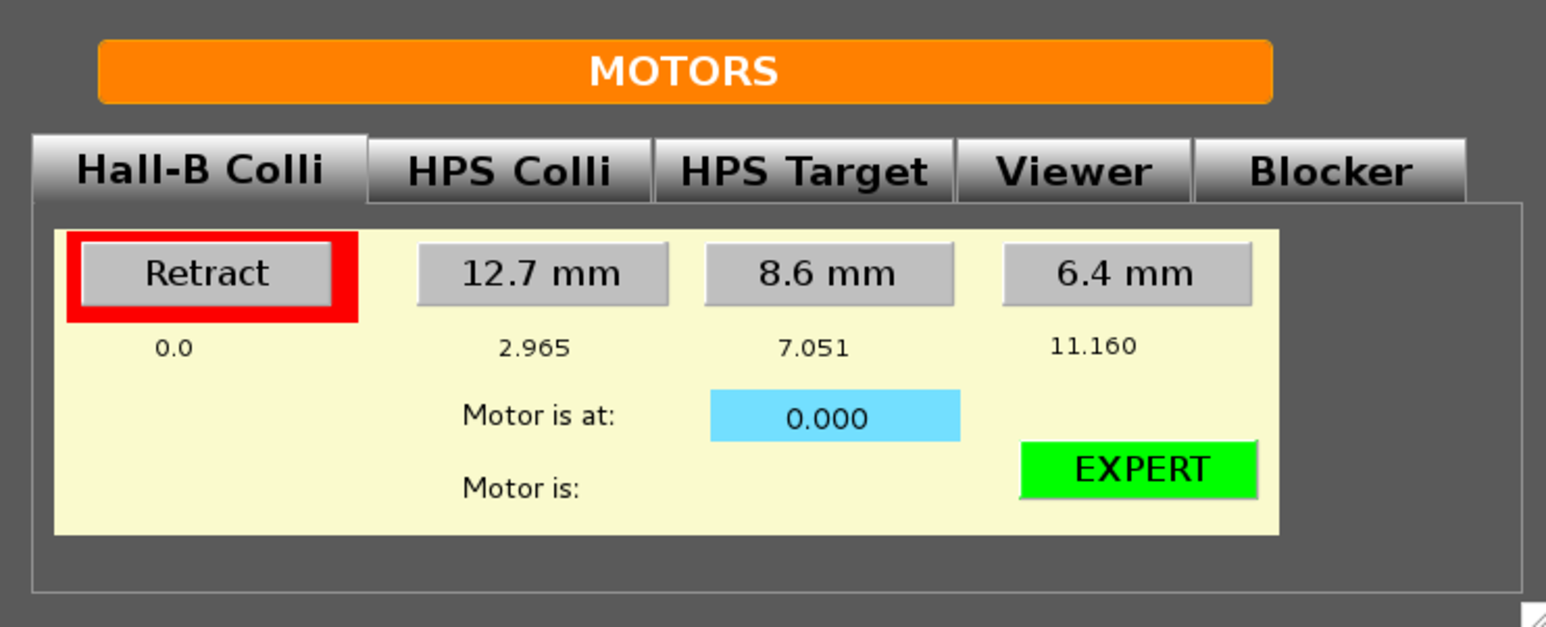
\includegraphics[scale=0.65]{collimator.pdf} \par}
\caption{The beam GUI to operate collimator and beam blocker. \label{fig:beamblocker}}
\end{figure}


\clearpage

\subsection{\bf Target}
\indent

The Hall-B cryo target from $6$ GeV era is used for the CLAS12. The main differences are larger diameter target cell and the longer supply pipes from condenser to the target. In anticipation of larger beam sizes at high energies ($> 3$ pass), target cell diameter is designed to be $20$ mm and the thin portion of the cell windows ($30~\mu$m thick aluminum) $10$ mm in diameter. Figure \ref{target} shows design rendering of the CLAS cryo target inside the foam scattering chamber. Control of the target, filling and emptying, will be done using {\it Target PC}. Operator should follow special instructions for the target operations. For monitoring, the target temperature, pressure, and the buffer dewar liquid level are displayed on the Main Control and Monitoring GUI, Figure \ref{fig:scaler}. 

\begin{figure}[ht!]
\centering
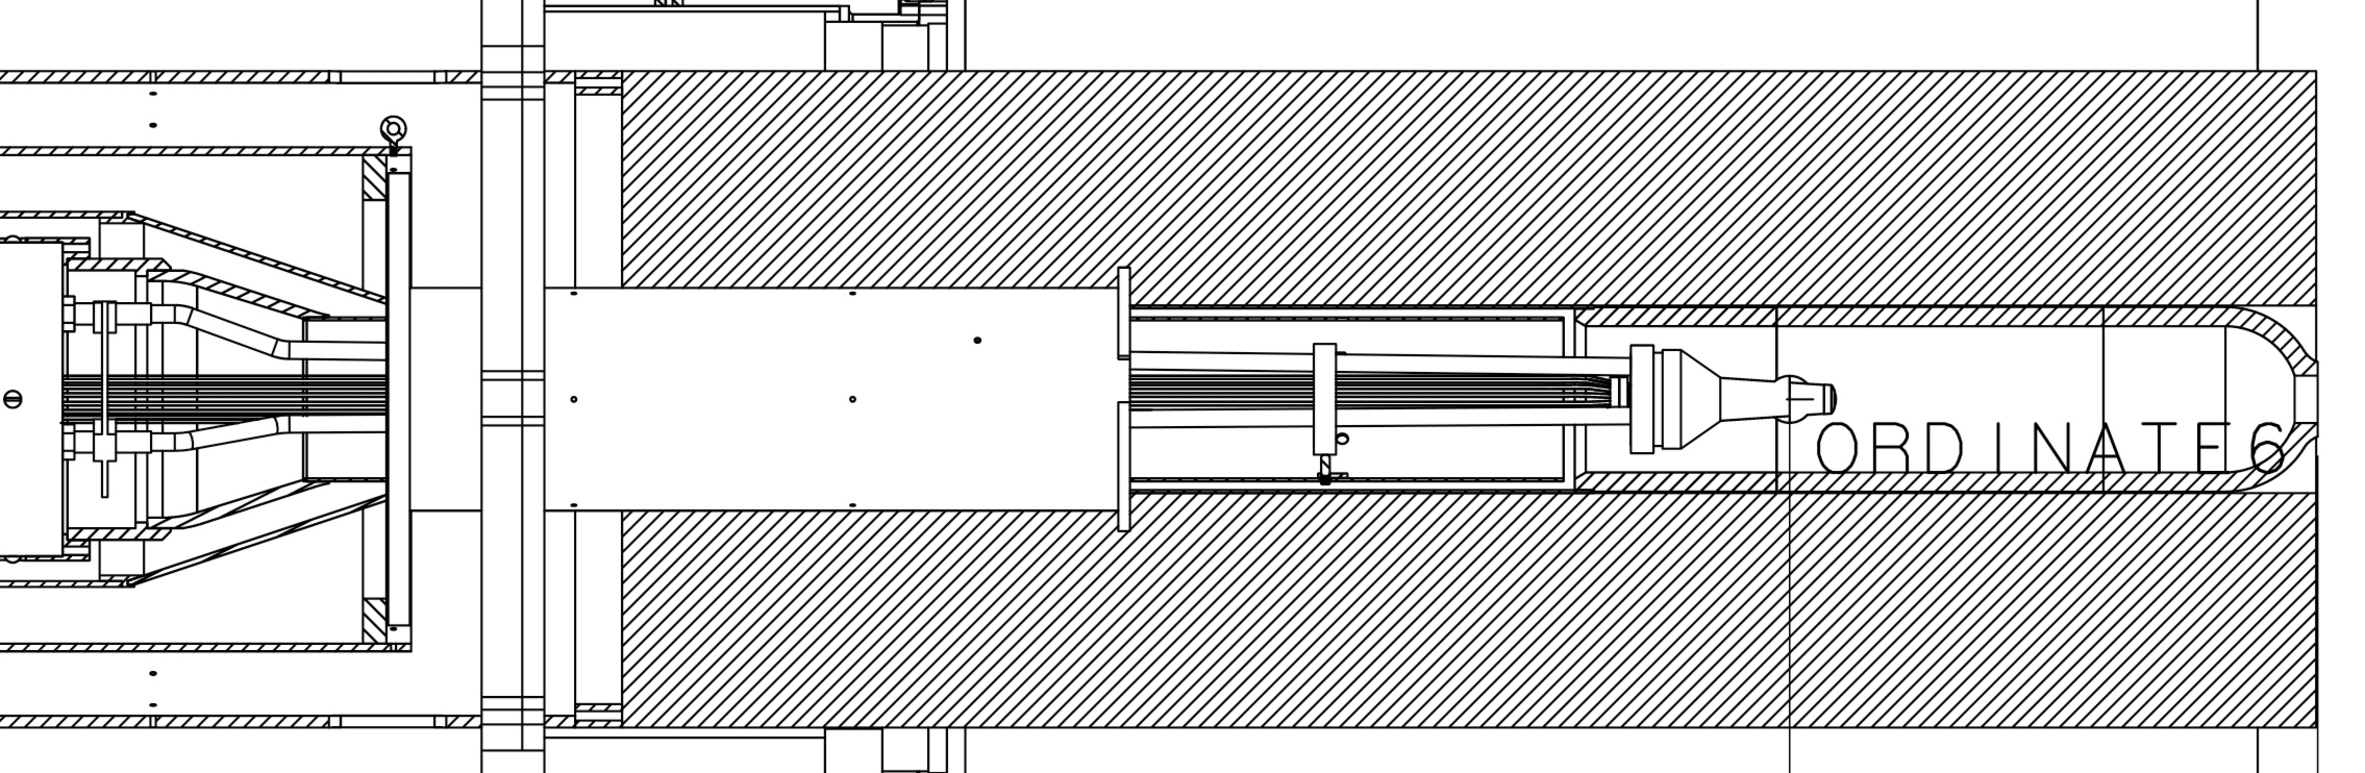
\includegraphics[width=1.\textwidth]{target.pdf}
\caption{Hall B cryo target and scattering chamber. }%The $20~\mu$m thick aluminum target cell windows are shown in red.}
\label{target}
\end{figure}

\clearpage

\begin{flushleft}
{\bf {\Large Appendix}}
\end{flushleft}

\section {Establishing beam for physics}
\indent

Establishing production quality electron beam for experiments in Hall B is a two step process. 

\subsection{Beam to tagger-yoke dump}
\indent

The initial tune is done at low currents, $<10$ nA, with dumping the beam on the "tagger-yoke dump", a dump in the tagger dipole magnet yoke, before hall proper. Beam is deflected down to this intermediate dump by the tagger dipole magnet \cite{tagger}. The tagger dipole power supply set current relates to the beam energy as \cite{yokedump}:
\begin{eqnarray}
I(A)~=~43.491\times E(GeV)-0.076
\end{eqnarray}

In this first step:
\begin{itemize}
\item the CLAS12 detectors (especially tracking detectors) must be OFF 
\item all halo counters must be ON
\item masked the halo counters (upstream, midstream, BOM and downstream) in beam Fast Shut Down (FSD) system 
\item the "blank" collimator with no hole is on the beam
\item the CLAS12 solenoid and torus magnets are energized (or can be be energized while beam tune is in progress)
\end{itemize}

The beam with required profile and trajectory is established by MCC ops using correctors and quadrupoles on 2C line, while monitored by Hall-B shift crew using the wire harps and the nanoamp (nA) BPMs \cite{nA_BPM} at 2C21 and 2C24 girders in the upstream tunnel (see  Figure \ref{fig:belements}). There is a Yag viewer, ITV2C24, upstream of the tagger dipole, controlled by MCC, that may be used by MCC to verify position and profile of the beam. Hall-B shift personnel should work with MCC operator to establish required quality beam. All harp scans must be properly analyzed and logged into logbook. The beam tune is good when required parameters for the profile (x/y widths) and trajectory (x/y positions on various monitors) are achieved. These parameters will be written on the run wiki and/or on the white board in the counting house. Typically widths at 2C21 harp $\sigma_{x,y}\le 200~\mu$m, while at 2C24 (tagger) harp $\sigma_{x,y}\le 500-600~\mu$m. In general it is a good practice to check newly measured beam parameters against last good/acceptable tune.  

\begin{figure}[htb!]
\centering
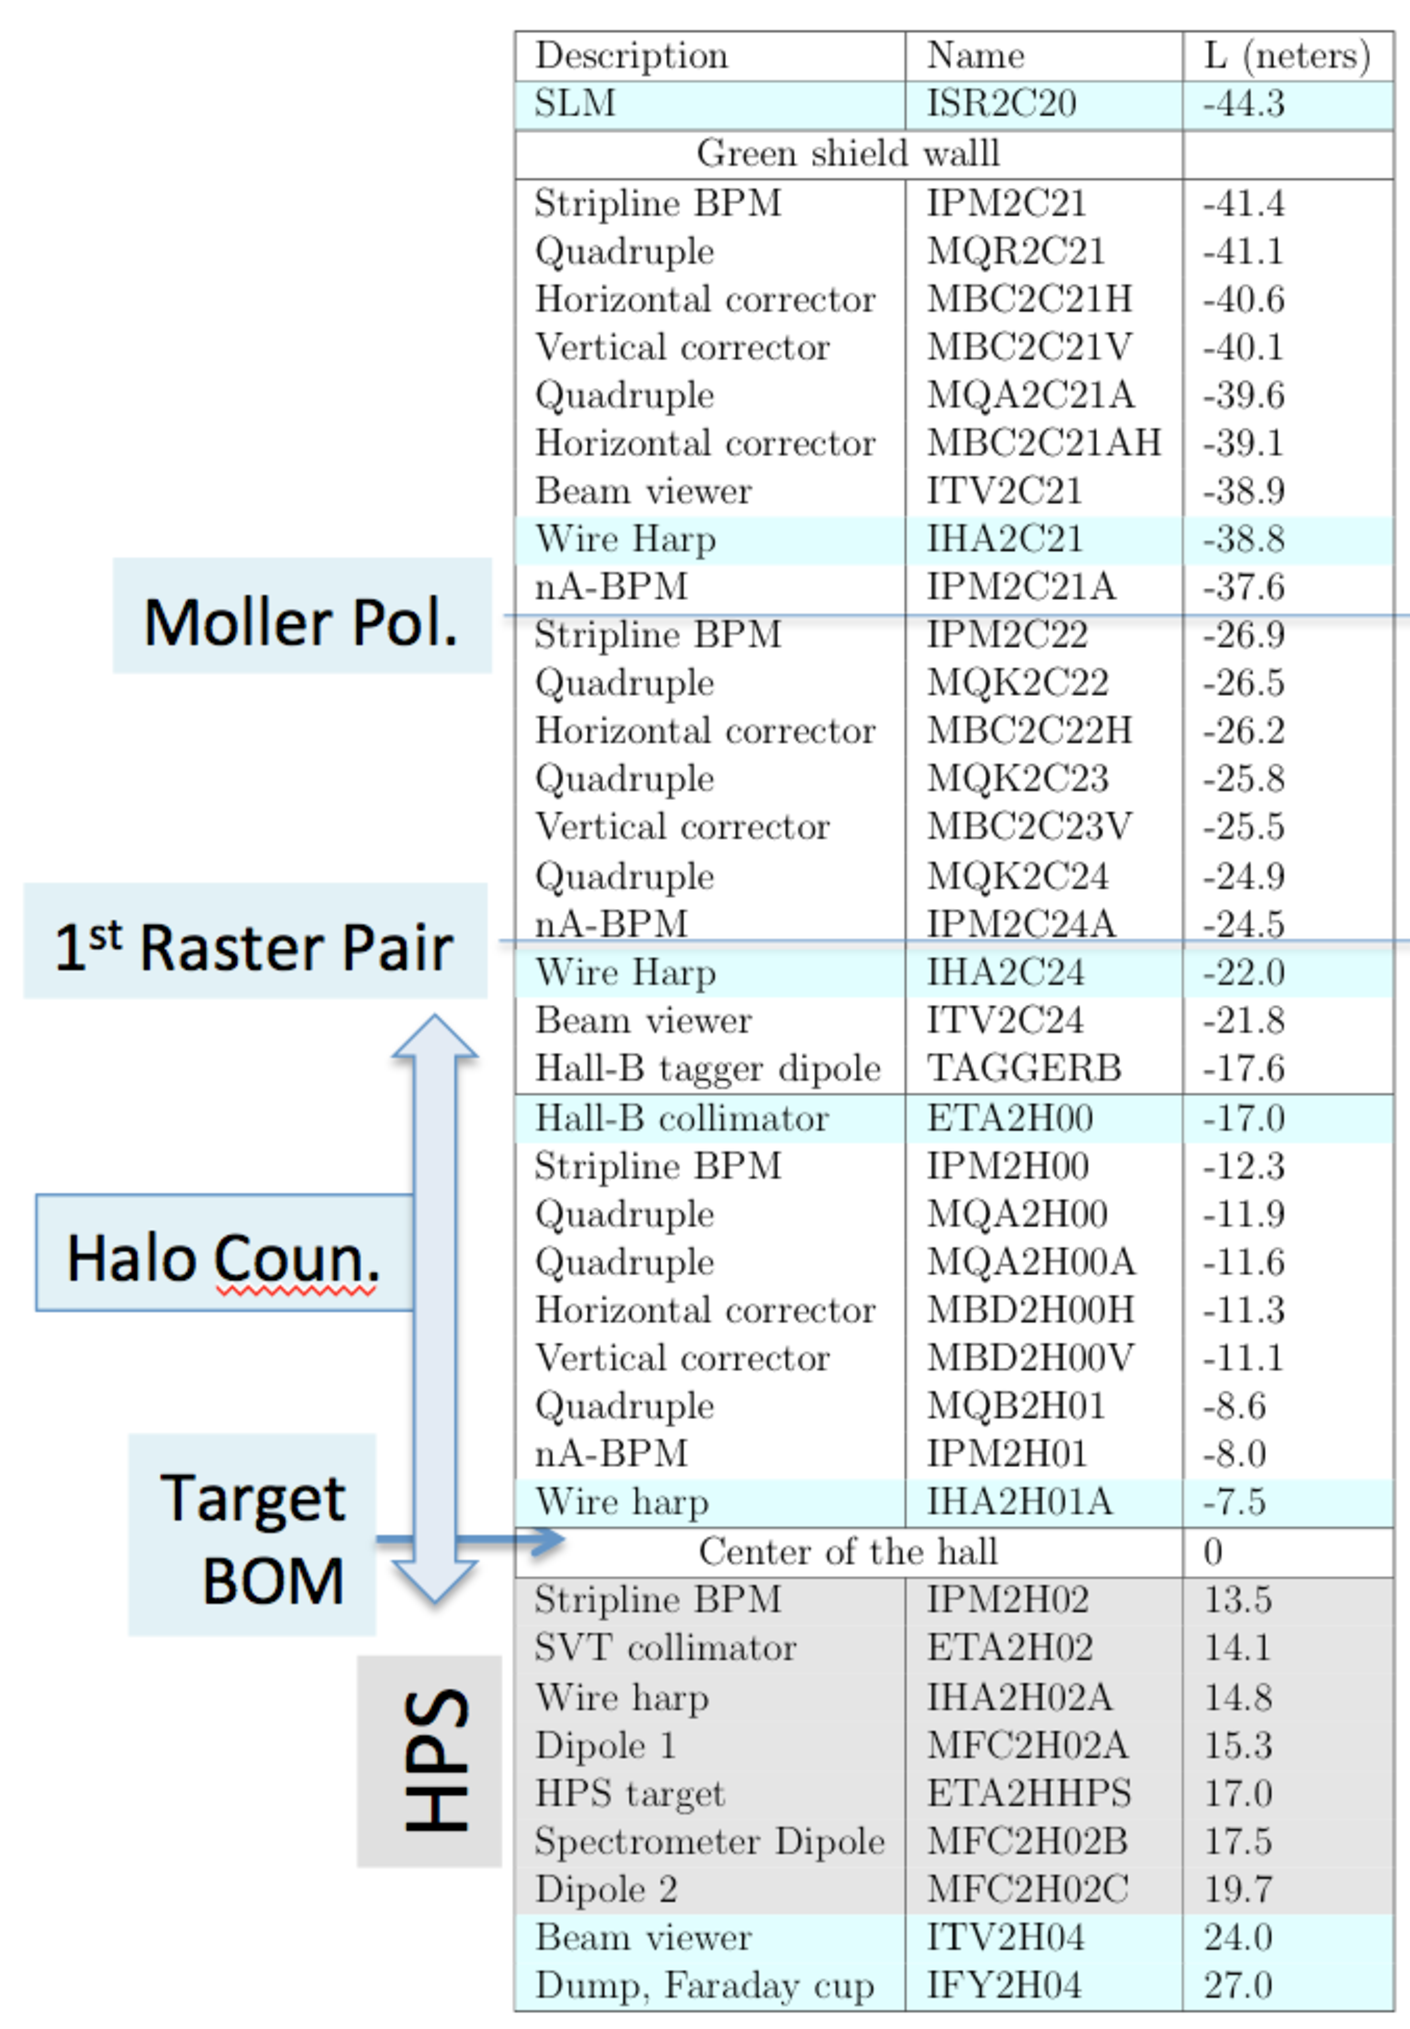
\includegraphics[width=0.8\textwidth]{beamline_elements.pdf}
\caption{Bemaline elements from the green shield wall to Faraday cup dump.}
\label{fig:belements}
\end{figure}

\clearpage
\subsection{Beam to Faraday cup}
\indent

The second step of establishing a physics quality beam starts after acceptable beam parameters have been achieved on the tagger-yoke dump. The following are steps for sending beam to CLAS12:
\begin{itemize}
\item tell MCC that beam is acceptable at the tagger
\item ask to take the beam away, and degauss and turn OFF the tagger magnet 
\item position $20$ mm diameter collimator on the beam 
\item set the halo counter FSD thresholds in to 1 MHz and the integration time interval to $50$ milliseconds
\item when ready ask MCC to send $\sim 5$ nA beam straight to the electron dump, at the end of the Hall B beamline where Faraday cup is located 
\item verify that beam goes to the dump 
\begin{description}
\item[a.] make sure beam is clearly visible on the downstream viewer, use Chromox screen\footnote{At low energies beam spot may not be clearly visible at 5 nA}. Beam should be within $10$ mm (2-tick marks) around the center 
\item[b.] make sure that Faraday cup beam current reading and the beam currents on 2C21 and 2C24 BPMs are consistent (the difference  should not be more then few \%)
\end{description}
\end{itemize}

The beam profile and position adjustments on the target will be done using correctors and quadrupoles on 2C22/2C23/2C24 girders in the upstream tunnel and 2H00 girder in the hall (if needed). The last one is the closest to the target ($\sim 10$m upstream) and will be used to focus beam at the target location to achieve required size (preferably $<300~\mu$m). The profile and position of the beam on the CLAS12 target will be checked using a 3-wire harp 2H01A mounted about $\sim 7$ meters upstream of the CLAS12 target and 2H01 nA BPM (stripline BPM on 2H00 will not work at low currents). The 2H01A harp measures the beam profile and its projected position along x-, y-, and $45^\circ$ axes. After physics quality beam is established based on the profile, beam position on either the cryo target cell or any of CLAS12 detector component (e.g. FTcal) must be adjusted based on the lowest rates on the downstream halo counters and on BOM or symmetry of rates in the detector. Procedure for adjusting the beam on the target is the following:
\begin{itemize}
\item ask MCC operator to move beam on 2H01 BPM by 0.1 mm steps up and down, vertical direction
\item record rates on halo counters and on BOM for each step. Stop moving in the given direction when rates go more more than $\times 10$ from where you started 
\item analyze rates as a function of position, find a position on 2H01 corresponding to the mid point of the two extreme ends where rates were highest. Ask MCC operator to position the beam on that position on 2H01 nA BPM
\item  repeat everything for horizontal alignment, moving the beam to left and right 
\item set orbit lock using found vertical and horizontal positions on 2H01 
\end{itemize}

For adjusting the beam position to get symmetric rates on a detector, e.g. FTcal, move beam with small steps in x- and/or y- on 2H01 nA BPM until desired symmetry is achieved.  
\vspace{1.cm}

After high quality beam was established and properly aligned, the beam orbit lock system should be engaged. This system incorporates position readings from the BPMs (2H01 and 2H00 if currents are high enough) to regulate 
currents in the horizontal and vertical corrector dipoles to minimize beam motion at the target.  The final step in establishing the production running conditions is setting 
limits on the halo counter and BOM rates for FSD system. If beam moves unexpectedly and gets close to an obstacle, e.g. 
collimator walls or to the thick parts of the target cell, count rates on the beam halo monitors and on the BOM will increase. The appropriate rate limits will depend on actual run conditions and the target, and will be noted on the white board in the counting room and/or on the run wiki. General prescription for setting a limit for FSD input rate of N(Hz) for a trip time interval of $\delta t$ is:
\begin{eqnarray*}
N_{thr}=N+n_\sigma\times\sqrt{N\over{\delta t}}
\end{eqnarray*}
where $n_\sigma$ is how far from mean value we want the trip to acquire. For example, for $\delta t=5$ ms - the recommended value, $n_\sigma=5.$ will mean one false tripe every $5$ hour. In order to avoid frequent false trips and allow some overhead in average rate and possible smaller time interval, a recommended value is $n_\sigma=6$. Note, when beam is cleanly transported to Faraday cup, "Upstream" and "Midstream" halo counters should count $<10$ - $15$ Hz, for those FSD threshold should be set to $1000$. High rates ($\sim 100$ Hz) on these counters will indicate bed beam transport or a bleed-through from other halls and must be corrected.



\section{EXPERT procedure for beam polarization measurement using the M{\"o}ller polarimeter}

\subsection{Before start}

\begin{itemize}
\item Reasonable quality beam must be already present for Hall-B
\item Beam has to be terminated on the tagger-yoke dump
\item CLAS12 is OFF, especially sensitive detectors: HV on \textbf{Drift Chambers} and \textbf{SVT/MVT}
\end{itemize}
%\item Harps are in the retracted position.
%\item Beam current should be set  to $\le 10$ nA 

%The optimal beam current is a function of beam energy. More specific information may be available on the white board in the counting house or in the run period specific documentation on the run wiki. Regardless of what currents are specified on the White board or in this document, the ratio $Left\otimes Right$ accidentals to the true coincidence rate should be kept below 5\%. It may be necessary to adjust the HV on the Left and Right PMT's to achieve a low accidental rate, while maintaining a reasonable true coincidence rate.

\subsection{Setup }

\begin{enumerate}
\item Notify MCC that you are about to do M{\"o}ller run and \textbf{request
to take the beam to the tagger yoke beam dump} (they will need to take the beam
away and energize the tagger magnet), MCC will ask to change BTA setting to ``photon" 
\item Ask MCC to turn orbit locks off, and mask BOM and Halo Counters in FSD 
\item Turning ON the polarimeter is done from EPICS GUIs (for now multiple control GUIs in expert mode are used). \\
{\bf NOTE: BEAM SHOULD BE OFF DURING the SETUP of M{\"o}LLER POLARIMETER}\\
M{\"o}ller setup GUIs can be launched from the \textbf{Moeller} tab on the \emph{"clascss"} GUI. 
%\latex{\ref{moller_epics}} on page\pageref{{moller_epics} } shows the
%M{\o}ller system GUI before the hardware has been set up. 

\begin{enumerate}
\item the "Moeller Asym - All" GUI, see Fig.\ref{fig:mainmoller} contains all the helicity gated scalers, charge asymmetry, and the beam polarization\footnote{The polarization and charge asymmetry have GUIs their own, but for now this main GUI will be used.}. It has several controls for the measurement and monitoring: 
\begin{description}
\item[Buttons "Start", "Reset" and "Stop"] will start and stop acquisition of data or reset acquisition (clear scaler buffers). 
\item[The acquisition time] controls update frequency of scalers, measured polarization value, and the charge asymmetry value. It is recommended to have M{\"o}ller polarimeter acquisition time $>60$ seconds when taking the measurements. For practical reasons, at the start when charge asymmetry will need tuning (see below) time for the scaler update can be set to $\sim 10$ seconds. The time can be set either by typing a value in the box or moving the slider. 
\item[The "Attenuator Controls"] are to control beam charge asymmetry. By changing voltage on intensity attenuators (IA) one can equalizes intensity across helicity states. It is recommended to use "Global Offset" that will change voltage on all four IAs at the same amount. Desire charge asymmetry is $<0.1\%$ based on SLM. 
\end{description}

%Make sure that the integration time for the asymmetry scalers is set to 5 on the \emph{``asym''} GUI under \emph{``Beamline''}. If it is not, use the slider to set it to 5 (if the slider wont move, check ``IOC ACCESS'' on \emph``clascss'' GUI on clonsl) 

\begin{figure}
\begin{center}
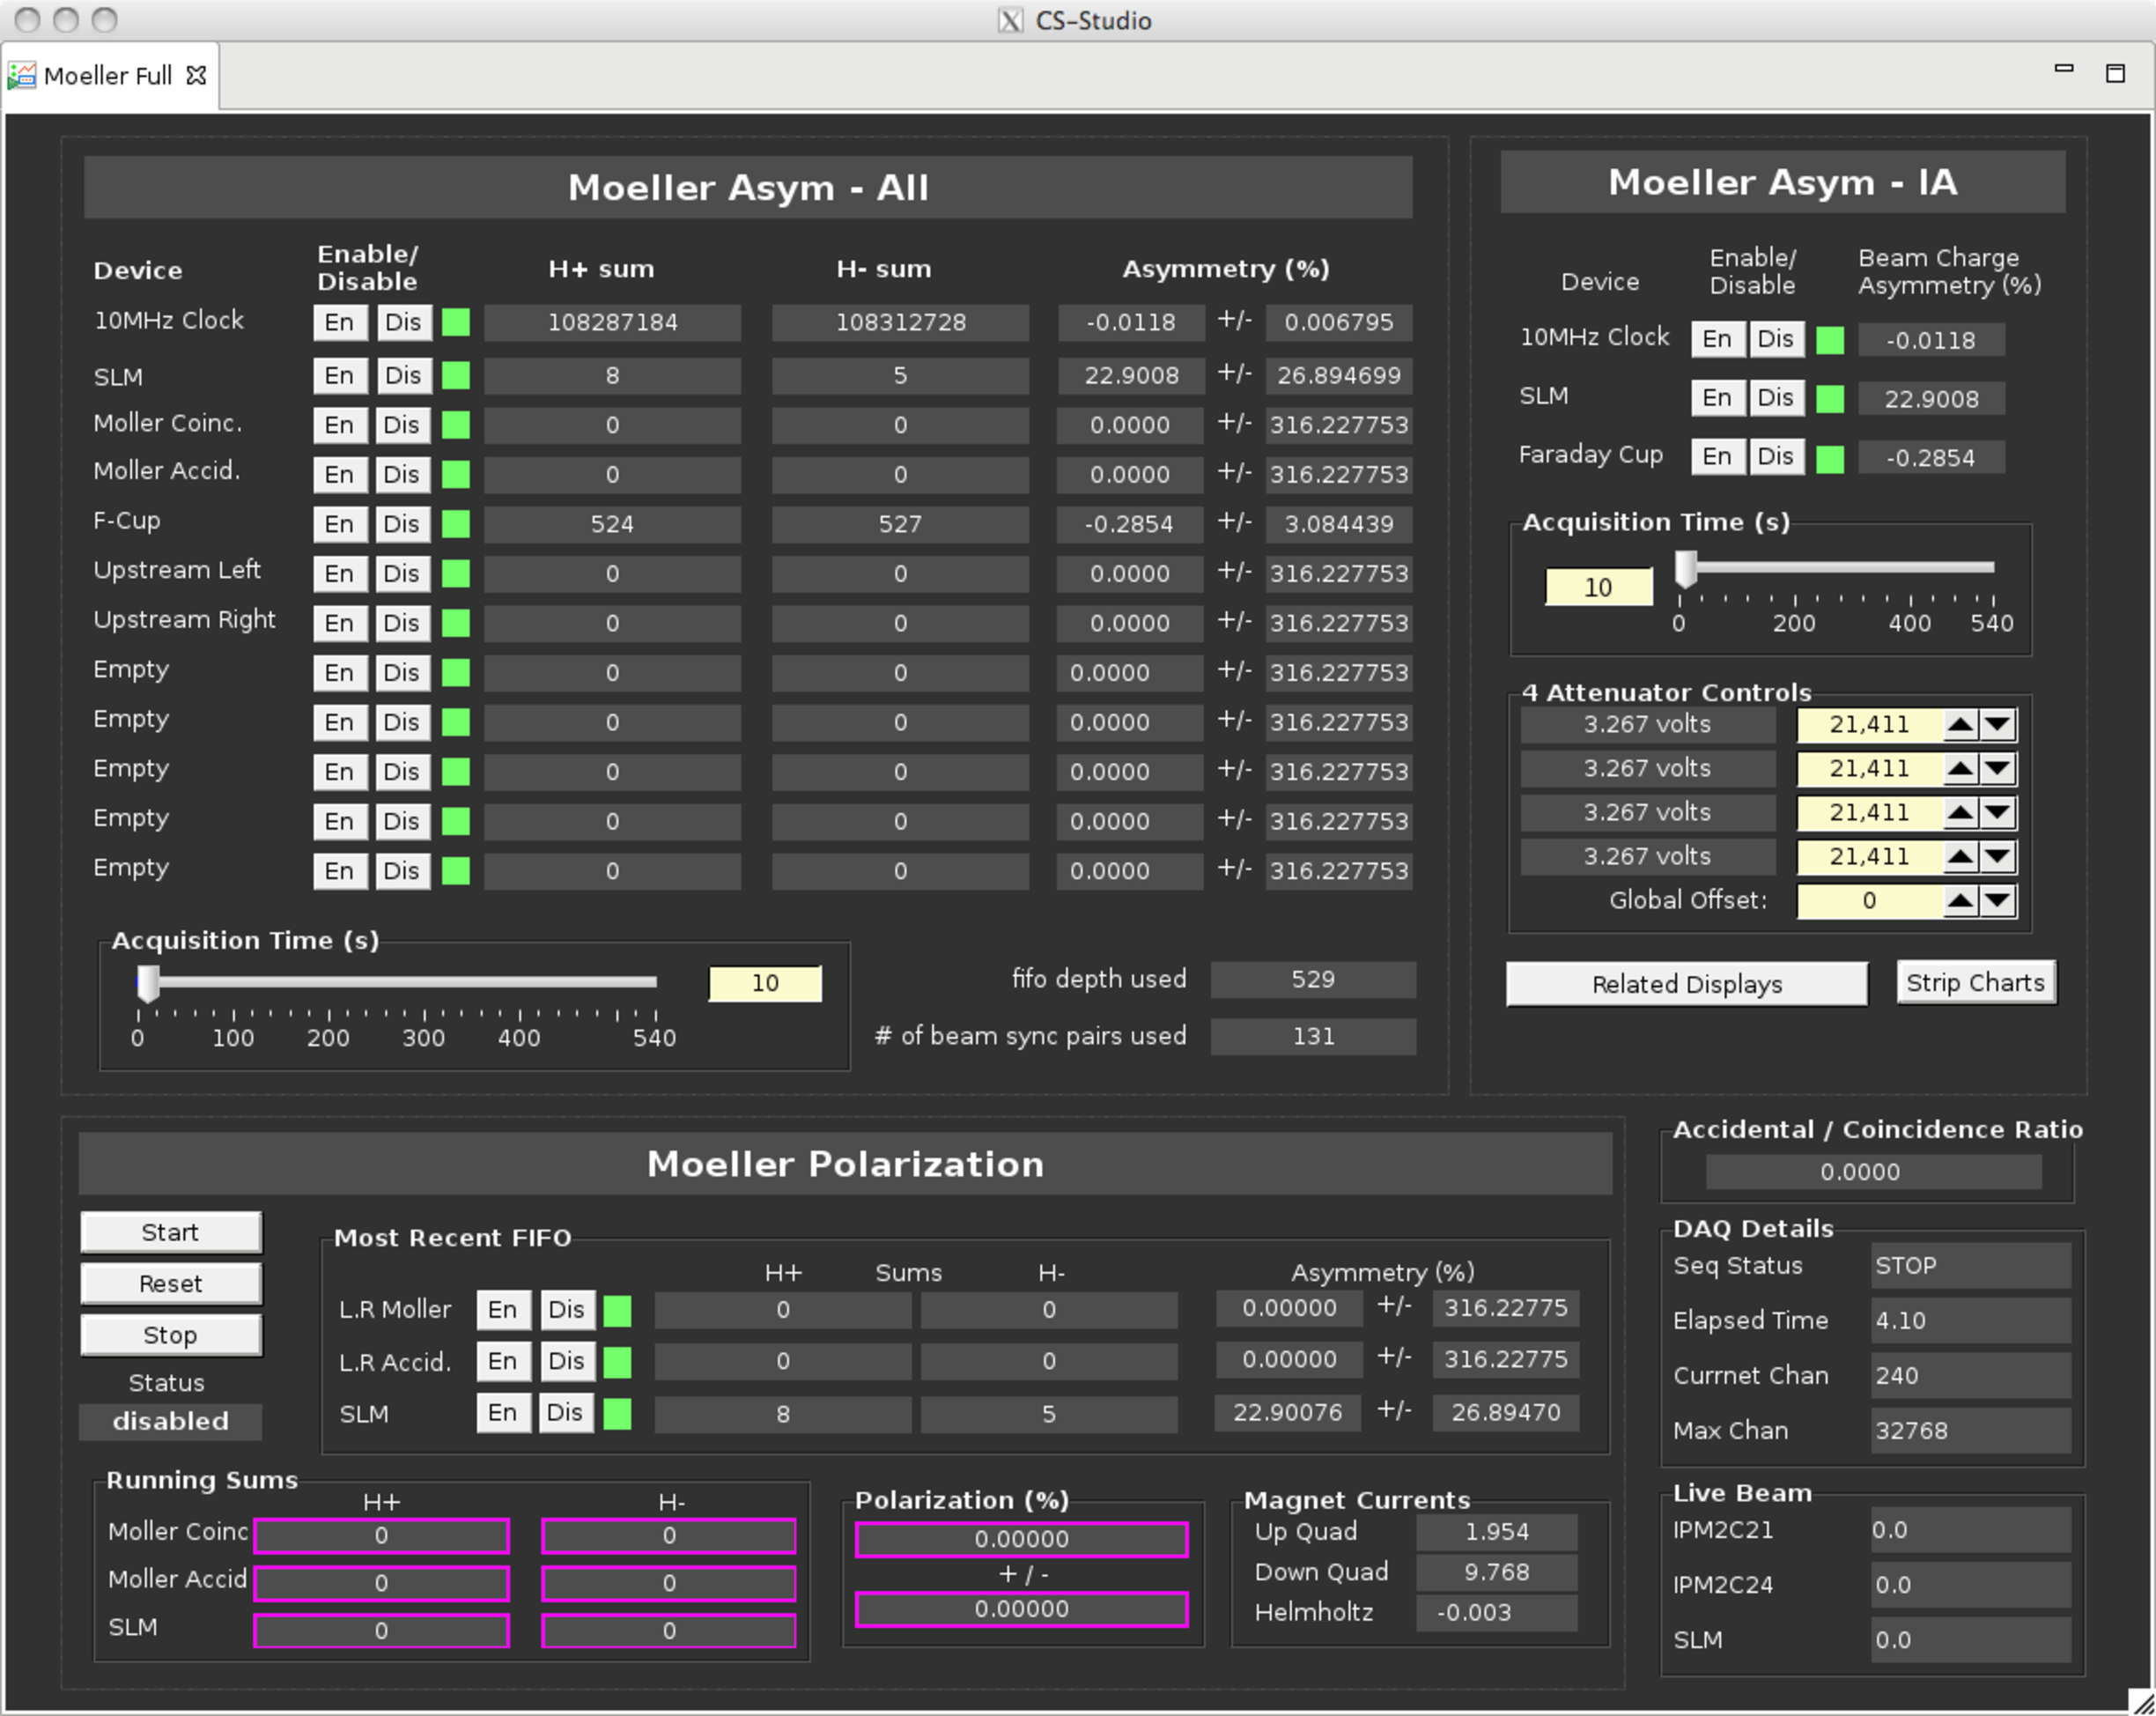
\includegraphics[width=0.8\textwidth]{moller_asym_all.pdf}
\caption{The main M{\"o}ller Epics expert GUI.}
\label{fig:mainmoller}
\end{center}
\end{figure}

\item The control for M{\"o}ller quadrupole power supplies are provided in "Moeller Quadrupoles" GUI, see Fig.\ref{moller_quad}. Power supplies will be turned ON and in remote before hall closing. From GUI one should first turn them on by pushing the "PS ON" buttons, then set the desire value for currents in "Current Setpoint" window. For $10.7$ GeV the suggested value for the quadrupoles is $3050$ A.

\begin{figure}
\begin{center}
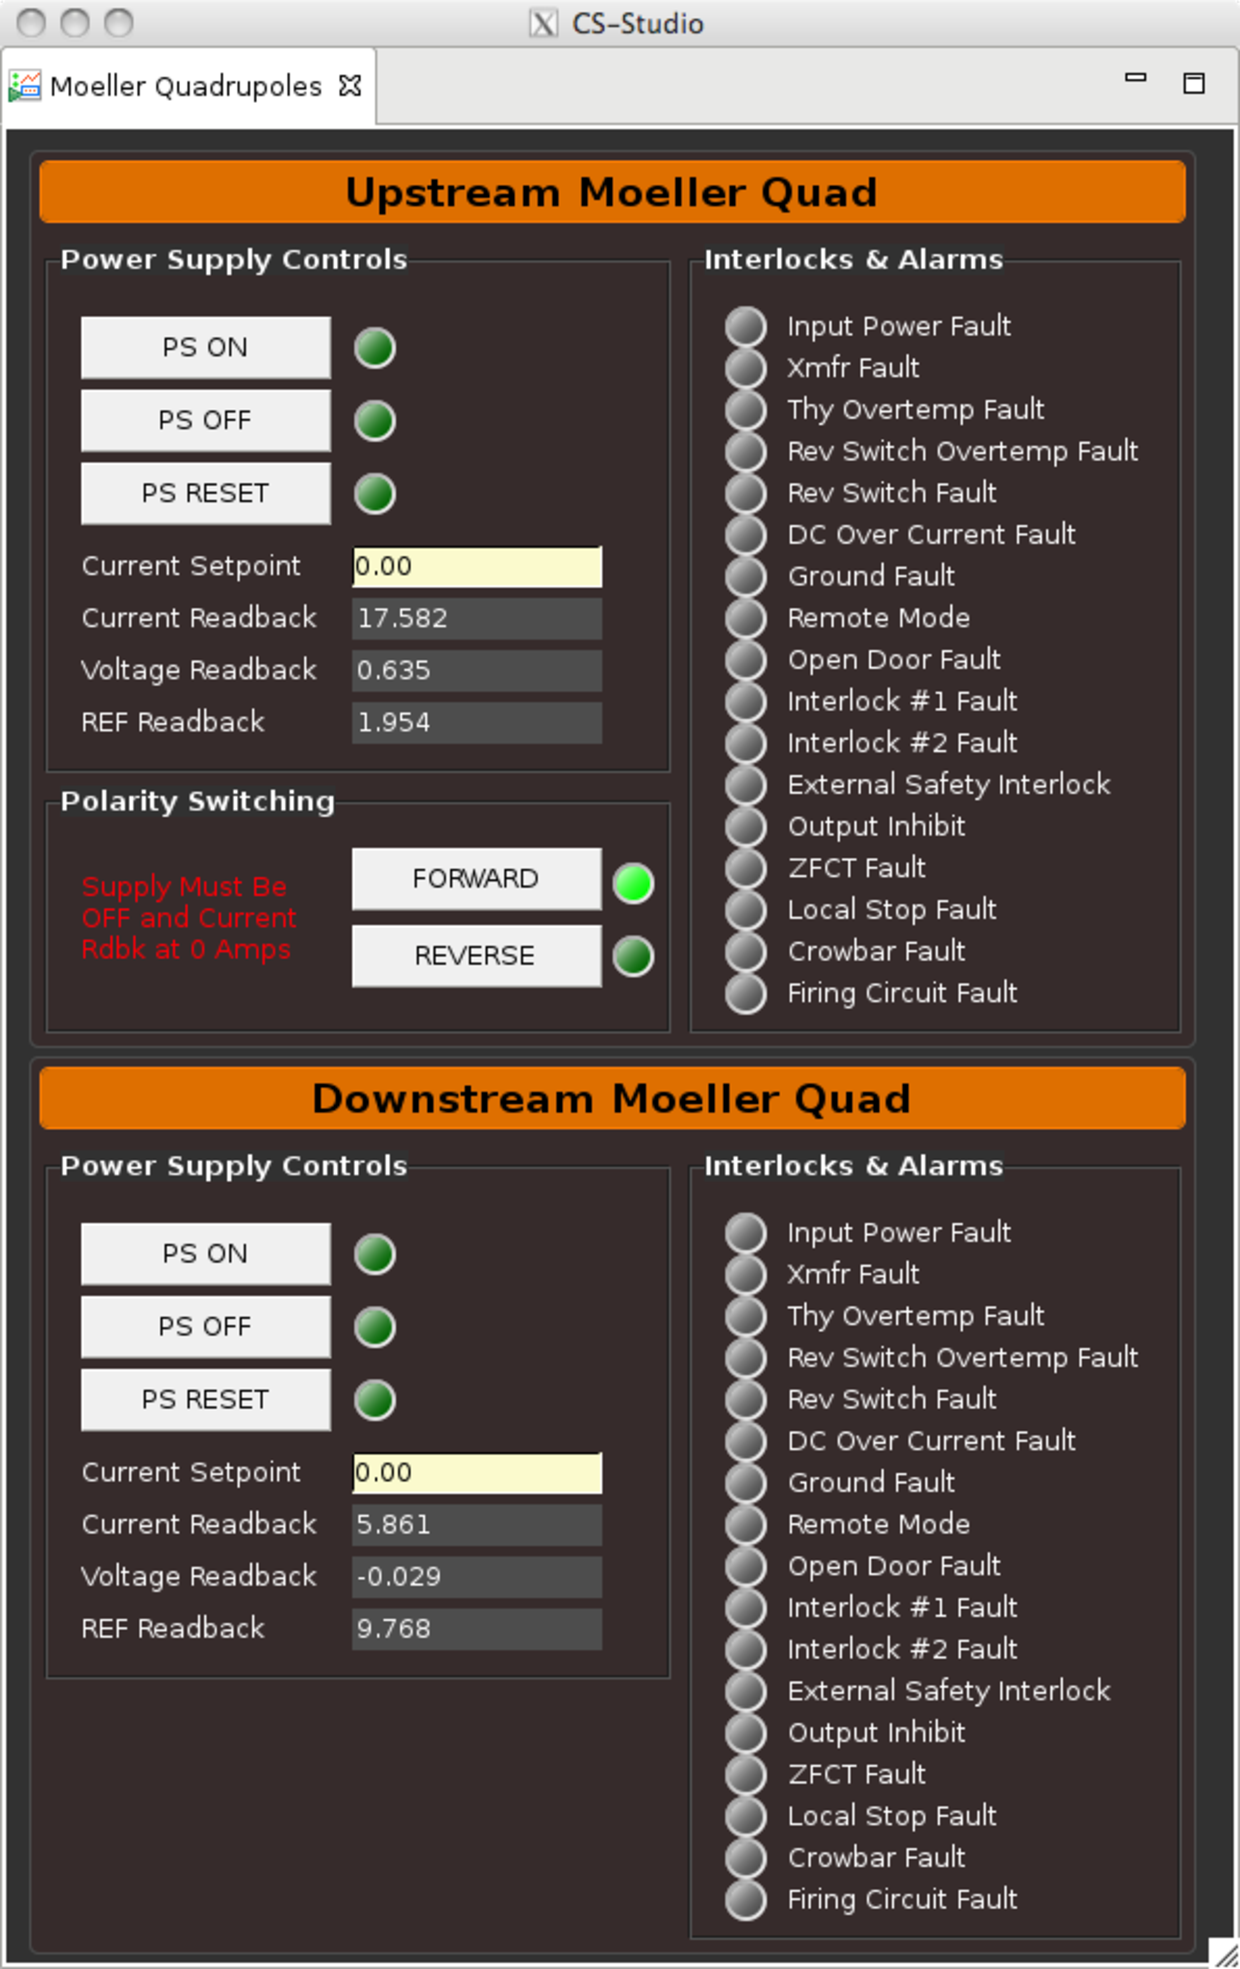
\includegraphics[width=0.75\textwidth]{moller_quad.pdf}
\caption{Control GUI for the M{\"o}ller quadrupole power supplies.}
\label{moller_quad}
\end{center}
\end{figure}


%Click \emph{``Configure M{\"o}ller Hardware''} button, near the top of the GUI, Figure \ref{moller_epics_setup}. This will start the following sequence of events:

%\begin{enumerate}
%\item SC HV Mainframes will be turned off.
%\item EC HV Mainframes will be turned off.
%\item Helmholtz Magnet will be energized in the Negative polarity.
%\item M{\"o}ller Target will be positioned to the \emph{LEFT} target position.
%\item M{\"o}ller Quadrupole magnets will be energized
%\item EPICS DAQ will be started
%\end{enumerate}
%\item Watch the text at the top of the GUI for informational guidance.

\item The target is polarized to its saturation by a longitudinal (along the beam) magnetic field generated using pair of Helmholtz coils. It is expected that the target will be saturated at $\sim 1.8$ A current in the coils. The recommended current for M{\"o}ller measurement is $3$ A. A GUI for power supply of Helmholtz coils, "Moeller Helmholtz PS" see Fig.\ref{moller_helm}, has two controls, button "STATE" defines state of the power supply. Typicaly it will be in "STANDBY" state when is not used. To energize coils first from the menu in "STATE" chose PS ON, then in "Current Setpoint", a white window, write the value, either $3$ or $-3$. Beam polarization measurements with both orientations the Helmholtz field is recommended to check systematics.    

\begin{figure}
\begin{center}
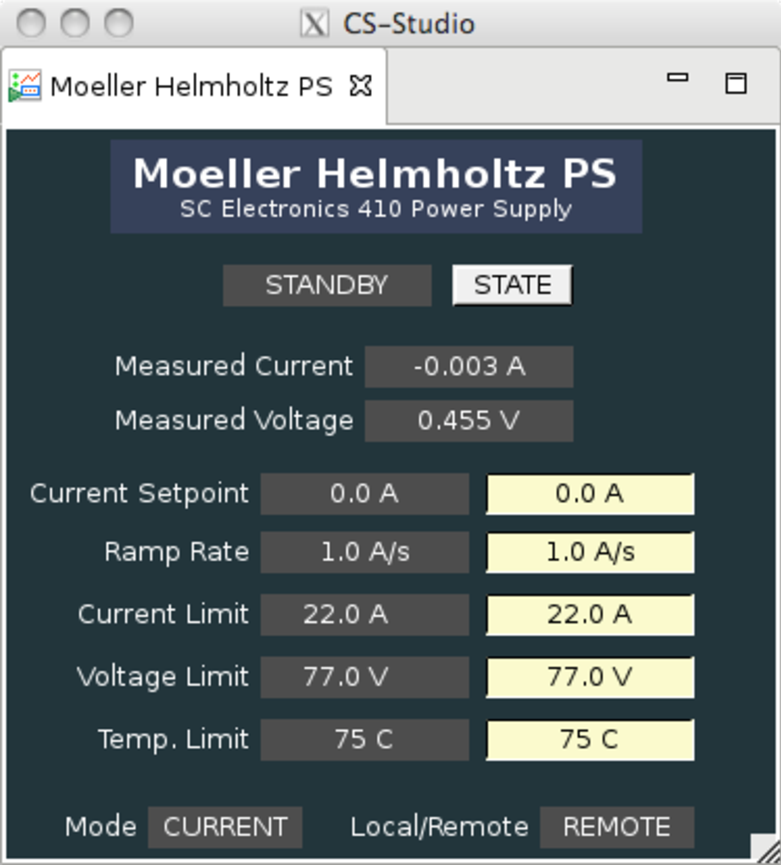
\includegraphics[width=0.65\textwidth]{moller_helmholtz.pdf}
\caption{Control GUI for the M{\"o}ller target Helmholtz coils power supply.}
\label{moller_helm}
\end{center}
\end{figure}
%\clearpage

\item a target control GUI, Fig.\ref{moller_target}, allows to position desired target on the beam. Left target is the recommended target for the measurements.

\begin{figure}
\begin{center}
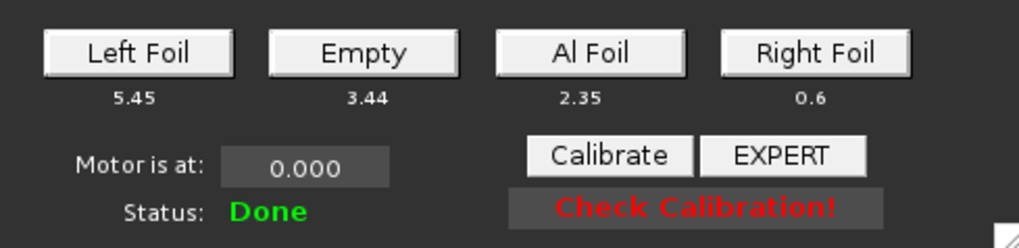
\includegraphics[width=0.65\textwidth]{moller_target.pdf}
\caption{Control GUI for the M{\"o}ller target.}
\label{moller_target}
\end{center}
\end{figure}

\end{enumerate}
%
%\clearpage

\item Once the tagger magnet is energized, M{\o}ller setup is UP and ready, request the beam current as specify for the given energy M{\o}ller measurements to be delivered\footnote{The optimal beam current is a function of beam energy.
More specific information may be available on the white board in the
counting house or in the run period specific documentation on the run wiki. Regardless
of what currents are specified on the white board or in this document,
the ratio $Left\otimes Right$ accidentals to the true coincidence
rate should be kept below 5\%. It may be necessary to adjust the
HV on the Left and Right PMT's to achieve a low accidental rate, while
maintaining a reasonable true rate.}, 
as measured by 2C21 nA BPM and/or SLM. Do
not use 2C24A since that BPM is located downstream of the M{\"o}ller setup. For $\sim 11$ GeV beam, if beam conditions are normal, as expected, the beam current should be $4$ nA. 

\end{enumerate}

%\clearpage
\subsection{Data Taking}
\indent
\begin{itemize}
\item 
To start a new run when DAQ is still running hit the "Reset" button on "Moeller Asym - All" GUI. If run was stoped hit the "Start" then "Reset". 
\item Run is complete when the error on the beam polarization on the GUI is below $\le 1.5\%$ absolute. Typically it takes about $45$ min to $60$ min to get the required accuracy (beam condition dependent). 
\item Make measurements with both positions of the half-wave plate,  "IN" and "OUT" (start the first measurement with whichever position it is, then do the second measurement with the other setting). 
\item If needed perform measurements with both polarity of the Helmholtz coils. 
\item Log every measurement by sending "Moeller Asym - All" GUI to logbook together with main scaler GUI to document beam currents, beam position, and halo counter rates. 
\end{itemize}

\subsection{Backing off M{\"o}ller setup out\label{moller close out}}

When done with the measurements:
\begin{itemize}
\item Do not forget to make a log entry including all details and the GUI! 

%Click the \emph{Backout Moller Hardware} button on the EPICS GUI to restore the hardware back to production running. 

\item Request MCC to take the beam away and \textbf{de-gauss the tagger
magnet if the next step is to send the beam to Faraday cup (usually it is).}

\item Turn off quadrupoles by setting $0$ in "Current Setpoint"s and then when current readback is at $\sim 0$ A push "PS OFF" button

\item Turn off Helmholtz coils by setting $0$ in the current "Current Setpoint" and change "STSTE" to "STANDBY" when "Measured Current" is $\sim 0$

\item Retract the target by pushing "Empty" button on the target GUI

\item Once tagger magnet is degaussed, restore beam to the Faraday Cup.

\item Turn ON CLAS12
\end{itemize}



%\subsubsection{Tips}

%\begin{enumerate}
%\item During a M{\"o}ller run the upstream PMTs labeled \char`\"{}up\char`\"{} and \char`\"{}down\char`\"{} may get activated. The half life is around 20 Minutes.~ MCC should ignore those PMTs for at least an hour. 
%\item MOLLER QUADS.~ At times the moller quads will not turn on.~ Using the Moller expert screens controls you can try a few things to get them on first try to click the \char`\"{}RESET\char`\"{} and \char`\"{}ON\char`\"{} buttons.~ Then you could try to click the \char`\"{}OFF\char`\"{} and then \char`\"{}ON\char`\"{} buttons.~ The readback value of the current should be close to the entered set value.
%\item Steering:~ Based on the beam tune, the moller quads may substantially deflect the beam.~ A deflection of 5 mm has been observed.~ 
%\item If the Moller PMT's do not come ON, try to reset them using the beamline HV GUI.
%\end{enumerate}



\begin{figure}[htb]
\centering
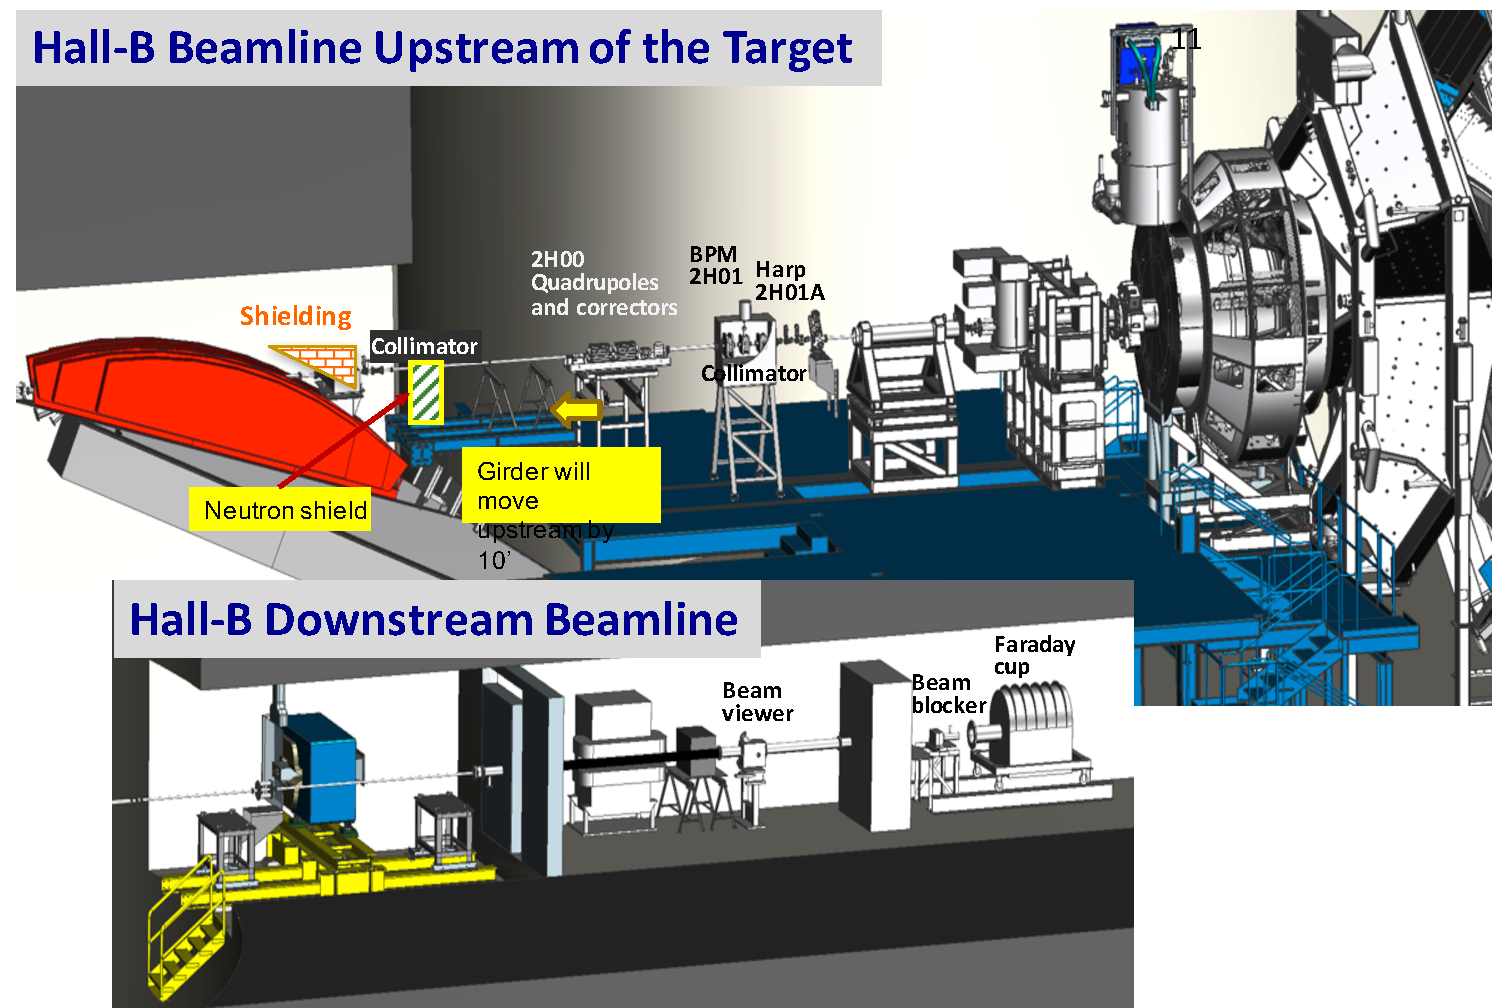
\includegraphics[angle=90,width=0.75\textwidth]{beamline_rendaring.pdf}
\caption{Hall-B beamline.}
\label{fig:bline}
\end{figure}


\begin{thebibliography}{00}
\bibitem{blocker} N. Dashyan and S. Stepanyan, CLAS12 Note 2016-004
\bibitem{2018-003} R. Paremuzyan and S. Stepanyan, CLAS12 Note 2018-003 (2018).
\bibitem{tagger} D. Sober et al., Nucl. Inst. and Meth. A 440, 263 (2000).
\bibitem{yokedump} https://clasweb.jlab.org/wiki/images/9/97/Beam\_on\_tagger.pdf
\bibitem{nA_BPM} M. Piller, et al., JLAB-ACC-99-30 (1998).
\end{thebibliography}


%


\end{document}
